\documentclass[11pt,a4paper]{article}
\usepackage[spanish,es-nodecimaldot]{babel}	% Utilizar español
\usepackage[utf8]{inputenc}					% Caracteres UTF-8
\usepackage{graphicx}						% Imagenes
\usepackage[hidelinks]{hyperref}			% Poner enlaces sin marcarlos en rojo
\usepackage{fancyhdr}						% Modificar encabezados y pies de pagina
\usepackage{float}							% Insertar figuras
\usepackage[textwidth=400pt]{geometry}		% Anchura de la pagina
\usepackage[nottoc]{tocbibind}				% Referencias (no incluir num pagina indice en Indice)
\usepackage{enumitem}						% Permitir enumerate con distintos simbolos
\usepackage[T1]{fontenc}					% Usar textsc en sections
\usepackage{amsmath}						% Símbolos matemáticos
\usepackage{fancyvrb} % verbatim replacement that allows latex
\usepackage{upquote} % Upright quotes for verbatim code
\usepackage{xcolor}


% Comando para poner el nombre de la asignatura
\newcommand{\asignatura}{Aprendizaje Automático}
\newcommand{\autor}{Vladislav Nikolov Vasilev}

% Configuracion de encabezados y pies de pagina
\pagestyle{fancy}
\lhead{\autor{}}
\rhead{\asignatura{}}
\lfoot{Grado en Ingeniería Informática}
\cfoot{}
\rfoot{\thepage}
\renewcommand{\headrulewidth}{0.4pt}		% Linea cabeza de pagina
\renewcommand{\footrulewidth}{0.4pt}		% Linea pie de pagina


    % Colors for the hyperref package
    \definecolor{urlcolor}{rgb}{0,.145,.698}
    \definecolor{linkcolor}{rgb}{.71,0.21,0.01}
    \definecolor{citecolor}{rgb}{.12,.54,.11}

    % ANSI colors
    \definecolor{ansi-black}{HTML}{3E424D}
    \definecolor{ansi-black-intense}{HTML}{282C36}
    \definecolor{ansi-red}{HTML}{E75C58}
    \definecolor{ansi-red-intense}{HTML}{B22B31}
    \definecolor{ansi-green}{HTML}{00A250}
    \definecolor{ansi-green-intense}{HTML}{007427}
    \definecolor{ansi-yellow}{HTML}{DDB62B}
    \definecolor{ansi-yellow-intense}{HTML}{B27D12}
    \definecolor{ansi-blue}{HTML}{208FFB}
    \definecolor{ansi-blue-intense}{HTML}{0065CA}
    \definecolor{ansi-magenta}{HTML}{D160C4}
    \definecolor{ansi-magenta-intense}{HTML}{A03196}
    \definecolor{ansi-cyan}{HTML}{60C6C8}
    \definecolor{ansi-cyan-intense}{HTML}{258F8F}
    \definecolor{ansi-white}{HTML}{C5C1B4}
    \definecolor{ansi-white-intense}{HTML}{A1A6B2}
    \definecolor{ansi-default-inverse-fg}{HTML}{FFFFFF}
    \definecolor{ansi-default-inverse-bg}{HTML}{000000}

    % commands and environments needed by pandoc snippets
    % extracted from the output of `pandoc -s`
    \providecommand{\tightlist}{%
      \setlength{\itemsep}{0pt}\setlength{\parskip}{0pt}}
    \DefineVerbatimEnvironment{Highlighting}{Verbatim}{commandchars=\\\{\}}
    % Add ',fontsize=\small' for more characters per line
    \newenvironment{Shaded}{}{}
    \newcommand{\KeywordTok}[1]{\textcolor[rgb]{0.00,0.44,0.13}{\textbf{{#1}}}}
    \newcommand{\DataTypeTok}[1]{\textcolor[rgb]{0.56,0.13,0.00}{{#1}}}
    \newcommand{\DecValTok}[1]{\textcolor[rgb]{0.25,0.63,0.44}{{#1}}}
    \newcommand{\BaseNTok}[1]{\textcolor[rgb]{0.25,0.63,0.44}{{#1}}}
    \newcommand{\FloatTok}[1]{\textcolor[rgb]{0.25,0.63,0.44}{{#1}}}
    \newcommand{\CharTok}[1]{\textcolor[rgb]{0.25,0.44,0.63}{{#1}}}
    \newcommand{\StringTok}[1]{\textcolor[rgb]{0.25,0.44,0.63}{{#1}}}
    \newcommand{\CommentTok}[1]{\textcolor[rgb]{0.38,0.63,0.69}{\textit{{#1}}}}
    \newcommand{\OtherTok}[1]{\textcolor[rgb]{0.00,0.44,0.13}{{#1}}}
    \newcommand{\AlertTok}[1]{\textcolor[rgb]{1.00,0.00,0.00}{\textbf{{#1}}}}
    \newcommand{\FunctionTok}[1]{\textcolor[rgb]{0.02,0.16,0.49}{{#1}}}
    \newcommand{\RegionMarkerTok}[1]{{#1}}
    \newcommand{\ErrorTok}[1]{\textcolor[rgb]{1.00,0.00,0.00}{\textbf{{#1}}}}
    \newcommand{\NormalTok}[1]{{#1}}
    
    % Additional commands for more recent versions of Pandoc
    \newcommand{\ConstantTok}[1]{\textcolor[rgb]{0.53,0.00,0.00}{{#1}}}
    \newcommand{\SpecialCharTok}[1]{\textcolor[rgb]{0.25,0.44,0.63}{{#1}}}
    \newcommand{\VerbatimStringTok}[1]{\textcolor[rgb]{0.25,0.44,0.63}{{#1}}}
    \newcommand{\SpecialStringTok}[1]{\textcolor[rgb]{0.73,0.40,0.53}{{#1}}}
    \newcommand{\ImportTok}[1]{{#1}}
    \newcommand{\DocumentationTok}[1]{\textcolor[rgb]{0.73,0.13,0.13}{\textit{{#1}}}}
    \newcommand{\AnnotationTok}[1]{\textcolor[rgb]{0.38,0.63,0.69}{\textbf{\textit{{#1}}}}}
    \newcommand{\CommentVarTok}[1]{\textcolor[rgb]{0.38,0.63,0.69}{\textbf{\textit{{#1}}}}}
    \newcommand{\VariableTok}[1]{\textcolor[rgb]{0.10,0.09,0.49}{{#1}}}
    \newcommand{\ControlFlowTok}[1]{\textcolor[rgb]{0.00,0.44,0.13}{\textbf{{#1}}}}
    \newcommand{\OperatorTok}[1]{\textcolor[rgb]{0.40,0.40,0.40}{{#1}}}
    \newcommand{\BuiltInTok}[1]{{#1}}
    \newcommand{\ExtensionTok}[1]{{#1}}
    \newcommand{\PreprocessorTok}[1]{\textcolor[rgb]{0.74,0.48,0.00}{{#1}}}
    \newcommand{\AttributeTok}[1]{\textcolor[rgb]{0.49,0.56,0.16}{{#1}}}
    \newcommand{\InformationTok}[1]{\textcolor[rgb]{0.38,0.63,0.69}{\textbf{\textit{{#1}}}}}
    \newcommand{\WarningTok}[1]{\textcolor[rgb]{0.38,0.63,0.69}{\textbf{\textit{{#1}}}}}
    
    
    % Define a nice break command that doesn't care if a line doesn't already
    % exist.
    \def\br{\hspace*{\fill} \\* }
    % Math Jax compatibility definitions
    \def\gt{>}
    \def\lt{<}
    \let\Oldtex\TeX
    \let\Oldlatex\LaTeX
    \renewcommand{\TeX}{\textrm{\Oldtex}}
    \renewcommand{\LaTeX}{\textrm{\Oldlatex}}
    % Document parameters
    % Document title
    \title{memoria}
    
    
    
    
    

    % Pygments definitions
    
\makeatletter
\def\PY@reset{\let\PY@it=\relax \let\PY@bf=\relax%
    \let\PY@ul=\relax \let\PY@tc=\relax%
    \let\PY@bc=\relax \let\PY@ff=\relax}
\def\PY@tok#1{\csname PY@tok@#1\endcsname}
\def\PY@toks#1+{\ifx\relax#1\empty\else%
    \PY@tok{#1}\expandafter\PY@toks\fi}
\def\PY@do#1{\PY@bc{\PY@tc{\PY@ul{%
    \PY@it{\PY@bf{\PY@ff{#1}}}}}}}
\def\PY#1#2{\PY@reset\PY@toks#1+\relax+\PY@do{#2}}

\expandafter\def\csname PY@tok@w\endcsname{\def\PY@tc##1{\textcolor[rgb]{0.73,0.73,0.73}{##1}}}
\expandafter\def\csname PY@tok@c\endcsname{\let\PY@it=\textit\def\PY@tc##1{\textcolor[rgb]{0.25,0.50,0.50}{##1}}}
\expandafter\def\csname PY@tok@cp\endcsname{\def\PY@tc##1{\textcolor[rgb]{0.74,0.48,0.00}{##1}}}
\expandafter\def\csname PY@tok@k\endcsname{\let\PY@bf=\textbf\def\PY@tc##1{\textcolor[rgb]{0.00,0.50,0.00}{##1}}}
\expandafter\def\csname PY@tok@kp\endcsname{\def\PY@tc##1{\textcolor[rgb]{0.00,0.50,0.00}{##1}}}
\expandafter\def\csname PY@tok@kt\endcsname{\def\PY@tc##1{\textcolor[rgb]{0.69,0.00,0.25}{##1}}}
\expandafter\def\csname PY@tok@o\endcsname{\def\PY@tc##1{\textcolor[rgb]{0.40,0.40,0.40}{##1}}}
\expandafter\def\csname PY@tok@ow\endcsname{\let\PY@bf=\textbf\def\PY@tc##1{\textcolor[rgb]{0.67,0.13,1.00}{##1}}}
\expandafter\def\csname PY@tok@nb\endcsname{\def\PY@tc##1{\textcolor[rgb]{0.00,0.50,0.00}{##1}}}
\expandafter\def\csname PY@tok@nf\endcsname{\def\PY@tc##1{\textcolor[rgb]{0.00,0.00,1.00}{##1}}}
\expandafter\def\csname PY@tok@nc\endcsname{\let\PY@bf=\textbf\def\PY@tc##1{\textcolor[rgb]{0.00,0.00,1.00}{##1}}}
\expandafter\def\csname PY@tok@nn\endcsname{\let\PY@bf=\textbf\def\PY@tc##1{\textcolor[rgb]{0.00,0.00,1.00}{##1}}}
\expandafter\def\csname PY@tok@ne\endcsname{\let\PY@bf=\textbf\def\PY@tc##1{\textcolor[rgb]{0.82,0.25,0.23}{##1}}}
\expandafter\def\csname PY@tok@nv\endcsname{\def\PY@tc##1{\textcolor[rgb]{0.10,0.09,0.49}{##1}}}
\expandafter\def\csname PY@tok@no\endcsname{\def\PY@tc##1{\textcolor[rgb]{0.53,0.00,0.00}{##1}}}
\expandafter\def\csname PY@tok@nl\endcsname{\def\PY@tc##1{\textcolor[rgb]{0.63,0.63,0.00}{##1}}}
\expandafter\def\csname PY@tok@ni\endcsname{\let\PY@bf=\textbf\def\PY@tc##1{\textcolor[rgb]{0.60,0.60,0.60}{##1}}}
\expandafter\def\csname PY@tok@na\endcsname{\def\PY@tc##1{\textcolor[rgb]{0.49,0.56,0.16}{##1}}}
\expandafter\def\csname PY@tok@nt\endcsname{\let\PY@bf=\textbf\def\PY@tc##1{\textcolor[rgb]{0.00,0.50,0.00}{##1}}}
\expandafter\def\csname PY@tok@nd\endcsname{\def\PY@tc##1{\textcolor[rgb]{0.67,0.13,1.00}{##1}}}
\expandafter\def\csname PY@tok@s\endcsname{\def\PY@tc##1{\textcolor[rgb]{0.73,0.13,0.13}{##1}}}
\expandafter\def\csname PY@tok@sd\endcsname{\let\PY@it=\textit\def\PY@tc##1{\textcolor[rgb]{0.73,0.13,0.13}{##1}}}
\expandafter\def\csname PY@tok@si\endcsname{\let\PY@bf=\textbf\def\PY@tc##1{\textcolor[rgb]{0.73,0.40,0.53}{##1}}}
\expandafter\def\csname PY@tok@se\endcsname{\let\PY@bf=\textbf\def\PY@tc##1{\textcolor[rgb]{0.73,0.40,0.13}{##1}}}
\expandafter\def\csname PY@tok@sr\endcsname{\def\PY@tc##1{\textcolor[rgb]{0.73,0.40,0.53}{##1}}}
\expandafter\def\csname PY@tok@ss\endcsname{\def\PY@tc##1{\textcolor[rgb]{0.10,0.09,0.49}{##1}}}
\expandafter\def\csname PY@tok@sx\endcsname{\def\PY@tc##1{\textcolor[rgb]{0.00,0.50,0.00}{##1}}}
\expandafter\def\csname PY@tok@m\endcsname{\def\PY@tc##1{\textcolor[rgb]{0.40,0.40,0.40}{##1}}}
\expandafter\def\csname PY@tok@gh\endcsname{\let\PY@bf=\textbf\def\PY@tc##1{\textcolor[rgb]{0.00,0.00,0.50}{##1}}}
\expandafter\def\csname PY@tok@gu\endcsname{\let\PY@bf=\textbf\def\PY@tc##1{\textcolor[rgb]{0.50,0.00,0.50}{##1}}}
\expandafter\def\csname PY@tok@gd\endcsname{\def\PY@tc##1{\textcolor[rgb]{0.63,0.00,0.00}{##1}}}
\expandafter\def\csname PY@tok@gi\endcsname{\def\PY@tc##1{\textcolor[rgb]{0.00,0.63,0.00}{##1}}}
\expandafter\def\csname PY@tok@gr\endcsname{\def\PY@tc##1{\textcolor[rgb]{1.00,0.00,0.00}{##1}}}
\expandafter\def\csname PY@tok@ge\endcsname{\let\PY@it=\textit}
\expandafter\def\csname PY@tok@gs\endcsname{\let\PY@bf=\textbf}
\expandafter\def\csname PY@tok@gp\endcsname{\let\PY@bf=\textbf\def\PY@tc##1{\textcolor[rgb]{0.00,0.00,0.50}{##1}}}
\expandafter\def\csname PY@tok@go\endcsname{\def\PY@tc##1{\textcolor[rgb]{0.53,0.53,0.53}{##1}}}
\expandafter\def\csname PY@tok@gt\endcsname{\def\PY@tc##1{\textcolor[rgb]{0.00,0.27,0.87}{##1}}}
\expandafter\def\csname PY@tok@err\endcsname{\def\PY@bc##1{\setlength{\fboxsep}{0pt}\fcolorbox[rgb]{1.00,0.00,0.00}{1,1,1}{\strut ##1}}}
\expandafter\def\csname PY@tok@kc\endcsname{\let\PY@bf=\textbf\def\PY@tc##1{\textcolor[rgb]{0.00,0.50,0.00}{##1}}}
\expandafter\def\csname PY@tok@kd\endcsname{\let\PY@bf=\textbf\def\PY@tc##1{\textcolor[rgb]{0.00,0.50,0.00}{##1}}}
\expandafter\def\csname PY@tok@kn\endcsname{\let\PY@bf=\textbf\def\PY@tc##1{\textcolor[rgb]{0.00,0.50,0.00}{##1}}}
\expandafter\def\csname PY@tok@kr\endcsname{\let\PY@bf=\textbf\def\PY@tc##1{\textcolor[rgb]{0.00,0.50,0.00}{##1}}}
\expandafter\def\csname PY@tok@bp\endcsname{\def\PY@tc##1{\textcolor[rgb]{0.00,0.50,0.00}{##1}}}
\expandafter\def\csname PY@tok@fm\endcsname{\def\PY@tc##1{\textcolor[rgb]{0.00,0.00,1.00}{##1}}}
\expandafter\def\csname PY@tok@vc\endcsname{\def\PY@tc##1{\textcolor[rgb]{0.10,0.09,0.49}{##1}}}
\expandafter\def\csname PY@tok@vg\endcsname{\def\PY@tc##1{\textcolor[rgb]{0.10,0.09,0.49}{##1}}}
\expandafter\def\csname PY@tok@vi\endcsname{\def\PY@tc##1{\textcolor[rgb]{0.10,0.09,0.49}{##1}}}
\expandafter\def\csname PY@tok@vm\endcsname{\def\PY@tc##1{\textcolor[rgb]{0.10,0.09,0.49}{##1}}}
\expandafter\def\csname PY@tok@sa\endcsname{\def\PY@tc##1{\textcolor[rgb]{0.73,0.13,0.13}{##1}}}
\expandafter\def\csname PY@tok@sb\endcsname{\def\PY@tc##1{\textcolor[rgb]{0.73,0.13,0.13}{##1}}}
\expandafter\def\csname PY@tok@sc\endcsname{\def\PY@tc##1{\textcolor[rgb]{0.73,0.13,0.13}{##1}}}
\expandafter\def\csname PY@tok@dl\endcsname{\def\PY@tc##1{\textcolor[rgb]{0.73,0.13,0.13}{##1}}}
\expandafter\def\csname PY@tok@s2\endcsname{\def\PY@tc##1{\textcolor[rgb]{0.73,0.13,0.13}{##1}}}
\expandafter\def\csname PY@tok@sh\endcsname{\def\PY@tc##1{\textcolor[rgb]{0.73,0.13,0.13}{##1}}}
\expandafter\def\csname PY@tok@s1\endcsname{\def\PY@tc##1{\textcolor[rgb]{0.73,0.13,0.13}{##1}}}
\expandafter\def\csname PY@tok@mb\endcsname{\def\PY@tc##1{\textcolor[rgb]{0.40,0.40,0.40}{##1}}}
\expandafter\def\csname PY@tok@mf\endcsname{\def\PY@tc##1{\textcolor[rgb]{0.40,0.40,0.40}{##1}}}
\expandafter\def\csname PY@tok@mh\endcsname{\def\PY@tc##1{\textcolor[rgb]{0.40,0.40,0.40}{##1}}}
\expandafter\def\csname PY@tok@mi\endcsname{\def\PY@tc##1{\textcolor[rgb]{0.40,0.40,0.40}{##1}}}
\expandafter\def\csname PY@tok@il\endcsname{\def\PY@tc##1{\textcolor[rgb]{0.40,0.40,0.40}{##1}}}
\expandafter\def\csname PY@tok@mo\endcsname{\def\PY@tc##1{\textcolor[rgb]{0.40,0.40,0.40}{##1}}}
\expandafter\def\csname PY@tok@ch\endcsname{\let\PY@it=\textit\def\PY@tc##1{\textcolor[rgb]{0.25,0.50,0.50}{##1}}}
\expandafter\def\csname PY@tok@cm\endcsname{\let\PY@it=\textit\def\PY@tc##1{\textcolor[rgb]{0.25,0.50,0.50}{##1}}}
\expandafter\def\csname PY@tok@cpf\endcsname{\let\PY@it=\textit\def\PY@tc##1{\textcolor[rgb]{0.25,0.50,0.50}{##1}}}
\expandafter\def\csname PY@tok@c1\endcsname{\let\PY@it=\textit\def\PY@tc##1{\textcolor[rgb]{0.25,0.50,0.50}{##1}}}
\expandafter\def\csname PY@tok@cs\endcsname{\let\PY@it=\textit\def\PY@tc##1{\textcolor[rgb]{0.25,0.50,0.50}{##1}}}

\def\PYZbs{\char`\\}
\def\PYZus{\char`\_}
\def\PYZob{\char`\{}
\def\PYZcb{\char`\}}
\def\PYZca{\char`\^}
\def\PYZam{\char`\&}
\def\PYZlt{\char`\<}
\def\PYZgt{\char`\>}
\def\PYZsh{\char`\#}
\def\PYZpc{\char`\%}
\def\PYZdl{\char`\$}
\def\PYZhy{\char`\-}
\def\PYZsq{\char`\'}
\def\PYZdq{\char`\"}
\def\PYZti{\char`\~}
% for compatibility with earlier versions
\def\PYZat{@}
\def\PYZlb{[}
\def\PYZrb{]}
\makeatother


    % Exact colors from NB
    \definecolor{incolor}{rgb}{0.0, 0.0, 0.5}
    \definecolor{outcolor}{rgb}{0.545, 0.0, 0.0}

\begin{document}
\pagenumbering{gobble}

% Pagina de titulo
\begin{titlepage}

\begin{minipage}{\textwidth}

\centering


\includegraphics[scale=0.5]{img/ugr.png}\\

\textsc{\Large \asignatura{}\\[0.2cm]}
\textsc{GRADO EN INGENIERÍA INFORMÁTICA}\\[1cm]

\noindent\rule[-1ex]{\textwidth}{1pt}\\[1.5ex]
\textsc{{\Huge PRÁCTICA 3\\[0.5ex]}}
\textsc{{\Large Programación\\}}
\noindent\rule[-1ex]{\textwidth}{2pt}\\[3.5ex]

\end{minipage}

\vspace{0.5cm}

\begin{minipage}{\textwidth}

\centering

\textbf{Autor}\\ {\autor{}}\\[2.5ex]
\textbf{Rama}\\ {Computación y Sistemas Inteligentes}\\[2.5ex]
\vspace{0.3cm}


\includegraphics[scale=0.3]{img/etsiit.jpeg}

\vspace{0.7cm}
\textsc{Escuela Técnica Superior de Ingenierías Informática y de Telecomunicación}\\
\vspace{1cm}
\textsc{Curso 2018-2019}
\end{minipage}
\end{titlepage}

\pagenumbering{arabic}
\tableofcontents
\thispagestyle{empty}				% No usar estilo en la pagina de indice

\newpage

\setlength{\parskip}{1em}

\section{\textsc{Problema de Regresión}}

\subsection{Descripción del problema}

En este problema vamos a trabajar con el conjunto de datos \textit{Airfoil Self-Noise}\cite{airfoil}, el cuál ha sido proporcionado
por la NASA, y contiene los resultados de haber realizado un conjunto de pruebas aerodinámicas y acústicas en un túnel de viento sobre
perfiles alares de dos y tres dimensiones.

El conjunto de datos está compuesto por 1503 filas y 6 columnas, los valores de las cuáles son todos números reales. Los datos de
las 5 primeras columnas se corresponden con los datos de entrada, y la última columna se corresponde con la información de salida.
A continuación se puede ver que representa cada uno de los atributos de forma ordenada:

\begin{enumerate}
	\item Frecuencia, medida en $Hz$.
	\item Ángulo de ataque (ángulo que forman la cuerda geométrica de un perfil alar con la dirección del aire incidente),
		  medida en grados.
	\item Longitud de la cuerda del perfil alar, medida en metros.
	\item Velocidad \textit{free-stream}, medida en metros por segundo. 
	\item Distancia de desplazamiento de succión, medida en metros.
	\item Nivel de presión sonora, medida en $dB$.
\end{enumerate}

 \subsection{Análisis de los datos}\label{anuxe1lisis-de-los-datos}

    Antes de comenzar con todo el proceso de elección y selección de un
modelo lineal, vamos a pararnos un momento para analizar los datos de
los que disponemos con el fin de obtener más información sobre el
problema.

Lo primero que tenemos que hacer es cargar los datos. Para ello, vamos a
usar una función genérica que nos permita leer ficheros de datos y
obtener un \emph{DataFrame} que podamos usar luego. Vamos a ver como
sería esta función:

\begin{Verbatim}[commandchars=\\\{\}]
{\color{incolor}In [{\color{incolor}1}]:} \PY{k+kn}{import} \PY{n+nn}{numpy} \PY{k}{as} \PY{n+nn}{np}
        \PY{k+kn}{import} \PY{n+nn}{pandas} \PY{k}{as} \PY{n+nn}{pd}
        \PY{k+kn}{import} \PY{n+nn}{matplotlib}\PY{n+nn}{.}\PY{n+nn}{pyplot} \PY{k}{as} \PY{n+nn}{plt}
        
        \PY{c+c1}{\PYZsh{} Establecer la semilla que vamos a utilizar}
        \PY{n}{np}\PY{o}{.}\PY{n}{random}\PY{o}{.}\PY{n}{seed}\PY{p}{(}\PY{l+m+mi}{1}\PY{p}{)}
        
        \PY{k}{def} \PY{n+nf}{read\PYZus{}data\PYZus{}values}\PY{p}{(}\PY{n}{in\PYZus{}file}\PY{p}{,} \PY{n}{separator}\PY{o}{=}\PY{k+kc}{None}\PY{p}{)}\PY{p}{:}
            \PY{l+s+sd}{\PYZdq{}\PYZdq{}\PYZdq{}}
        \PY{l+s+sd}{    Funcion para leer los datos de un archivo}
        \PY{l+s+sd}{    }
        \PY{l+s+sd}{    :param in\PYZus{}file Archivo de entrada}
        \PY{l+s+sd}{    :param separator Separador que se utiliza en el archivo}
        \PY{l+s+sd}{                     (por defecto None)}
        \PY{l+s+sd}{    }
        \PY{l+s+sd}{    :return Devuelve los datos leidos del archivo en un DataFrame}
        \PY{l+s+sd}{    \PYZdq{}\PYZdq{}\PYZdq{}}
            
            \PY{c+c1}{\PYZsh{} Cargar los datos en un DataFrame}
            \PY{c+c1}{\PYZsh{} Se indica que la primera columna no es el header}
            \PY{k}{if} \PY{n}{separator} \PY{o}{==} \PY{k+kc}{None}\PY{p}{:}
                \PY{n}{df} \PY{o}{=} \PY{n}{pd}\PY{o}{.}\PY{n}{read\PYZus{}csv}\PY{p}{(}\PY{n}{in\PYZus{}file}\PY{p}{,} \PY{n}{header}\PY{o}{=}\PY{k+kc}{None}\PY{p}{)}
            \PY{k}{else}\PY{p}{:}
                \PY{n}{df} \PY{o}{=} \PY{n}{pd}\PY{o}{.}\PY{n}{read\PYZus{}csv}\PY{p}{(}\PY{n}{in\PYZus{}file}\PY{p}{,} \PY{n}{sep}\PY{o}{=}\PY{n}{separator}\PY{p}{,} \PY{n}{header}\PY{o}{=}\PY{k+kc}{None}\PY{p}{)}
            
            \PY{k}{return} \PY{n}{df}
\end{Verbatim}

    Con la función ya mostrada, vamos a cargar los datos y mostrar los
primeros valores de la muestra, para tener una idea de como serán los
datos:

    \begin{Verbatim}[commandchars=\\\{\}]
{\color{incolor}In [{\color{incolor}2}]:} \PY{n}{df} \PY{o}{=} \PY{n}{read\PYZus{}data\PYZus{}values}\PY{p}{(}\PY{l+s+s1}{\PYZsq{}}\PY{l+s+s1}{datos/airfoil\PYZus{}self\PYZus{}noise.dat}\PY{l+s+s1}{\PYZsq{}}\PY{p}{,} 
			       \PY{n}{separator}\PY{o}{=}\PY{l+s+s1}{\PYZsq{}}\PY{l+s+se}{\PYZbs{}t}\PY{l+s+s1}{\PYZsq{}}\PY{p}{)}
        
        \PY{c+c1}{\PYZsh{} Asignamos nombres a las columnas (según los atributos)}
        \PY{n}{column\PYZus{}names} \PY{o}{=} \PY{p}{[}\PY{l+s+s1}{\PYZsq{}}\PY{l+s+s1}{Frequency}\PY{l+s+s1}{\PYZsq{}}\PY{p}{,} \PY{l+s+s1}{\PYZsq{}}\PY{l+s+s1}{Angle of attack}\PY{l+s+s1}{\PYZsq{}}\PY{p}{,} \PY{l+s+s1}{\PYZsq{}}\PY{l+s+s1}{Chord length}\PY{l+s+s1}{\PYZsq{}}\PY{p}{,}
                        \PY{l+s+s1}{\PYZsq{}}\PY{l+s+s1}{Free\PYZhy{}stream velocity}\PY{l+s+s1}{\PYZsq{}}\PY{p}{,} \PY{l+s+s1}{\PYZsq{}}\PY{l+s+s1}{SSD thickness}\PY{l+s+s1}{\PYZsq{}}\PY{p}{,} 
                        \PY{l+s+s1}{\PYZsq{}}\PY{l+s+s1}{Sound Pressure}\PY{l+s+s1}{\PYZsq{}}\PY{p}{]}
        \PY{n}{df}\PY{o}{.}\PY{n}{columns} \PY{o}{=} \PY{n}{column\PYZus{}names}
        
        \PY{c+c1}{\PYZsh{} Mostrar primeros valores de los datos}
        \PY{n}{df}\PY{o}{.}\PY{n}{head}\PY{p}{(}\PY{p}{)}
\end{Verbatim}

\begin{figure}[H]
\centering
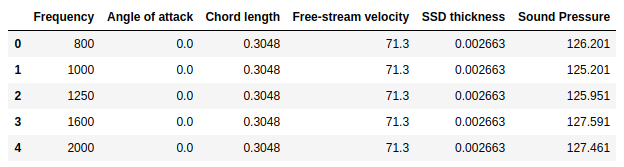
\includegraphics[scale=0.6]{img/train_head.png}
\caption{Tabla con las 5 primeras muestras del para el problema de regresión.}
\end{figure}

    Antes de proseguir, vamos a dividir los datos en los conjuntos de
training y test, ya que en este caso disponemos solo de un conjunto de
datos (no viene separado por defecto). Para esto, vamos a crear primero
una función que nos permita dividir los datos que tenemos en las
características (a lo que llamaremos \(\mathbf{X}\)) y las etiquetas (a
lo que llamaremos \(y\)). Una vez hecha esta separación, podremos
dividir los datos en los dos conjuntos anteriormente mencionados. Vamos
a hacer que el 80\% de los datos se quede en training y que el 20\% de
los datos esté en test. Por tanto, en resumidas cuentas, estamos
haciendo \emph{hold-out}, ya que nos quedamos con una parte de los datos
para poder estimar un E\(_{test}\) que nos permita acotar E\(_{out}\)
posteriormente. Esto tiene sus efectos negativos, como que por ejemplo
tengamos menos datos con los que entrenar y que los resultados pueden
ser un poco peores por este motivo, pero al menos tenemos una capacidad
para probar como de bueno es nuestro ajuste fuera de la muestra con la
que lo hemos entrenado.

Con esto dicho, vamos a ver como ser haría:

    \begin{Verbatim}[commandchars=\\\{\}]
{\color{incolor}In [{\color{incolor}3}]:} \PY{c+c1}{\PYZsh{} Función para dividir los datos en train y test}
        \PY{k+kn}{from} \PY{n+nn}{sklearn}\PY{n+nn}{.}\PY{n+nn}{model\PYZus{}selection} \PY{k}{import} \PY{n}{train\PYZus{}test\PYZus{}split}
        
        \PY{k}{def} \PY{n+nf}{divide\PYZus{}data\PYZus{}labels}\PY{p}{(}\PY{n}{input\PYZus{}data}\PY{p}{)}\PY{p}{:}
            \PY{l+s+sd}{\PYZdq{}\PYZdq{}\PYZdq{}}
        \PY{l+s+sd}{    Funcion que divide una muestra en los datos y las etiquetas}
        \PY{l+s+sd}{    }
        \PY{l+s+sd}{    :param input\PYZus{}data Conjunto de valores que se quieren separar}
        \PY{l+s+sd}{                      juntados en un DataFrame}
        \PY{l+s+sd}{    }
        \PY{l+s+sd}{    :return Devuelve los datos y las etiquetas}
        \PY{l+s+sd}{    \PYZdq{}\PYZdq{}\PYZdq{}}
            
            \PY{c+c1}{\PYZsh{}Obtener los valores}
            \PY{n}{values} \PY{o}{=} \PY{n}{input\PYZus{}data}\PY{o}{.}\PY{n}{values}
            
            \PY{c+c1}{\PYZsh{} Obtener datos y etiquetas}
            \PY{n}{X} \PY{o}{=} \PY{n}{values}\PY{p}{[}\PY{p}{:}\PY{p}{,} \PY{p}{:}\PY{o}{\PYZhy{}}\PY{l+m+mi}{1}\PY{p}{]}
            \PY{n}{y} \PY{o}{=} \PY{n}{values}\PY{p}{[}\PY{p}{:}\PY{p}{,} \PY{o}{\PYZhy{}}\PY{l+m+mi}{1}\PY{p}{]}
            
            \PY{k}{return} \PY{n}{X}\PY{p}{,} \PY{n}{y}
        
        \PY{c+c1}{\PYZsh{} Obtener valores X, Y}
        \PY{n}{X}\PY{p}{,} \PY{n}{y} \PY{o}{=} \PY{n}{divide\PYZus{}data\PYZus{}labels}\PY{p}{(}\PY{n}{df}\PY{p}{)}
        
        \PY{c+c1}{\PYZsh{} Dividir los datos en training y test}
        \PY{n}{X\PYZus{}train}\PY{p}{,} \PY{n}{X\PYZus{}test}\PY{p}{,} \PY{n}{y\PYZus{}train}\PY{p}{,} \PY{n}{y\PYZus{}test} \PY{o}{=} \PY{n}{train\PYZus{}test\PYZus{}split}\PY{p}{(}\PY{n}{X}\PY{p}{,} \PY{n}{y}\PY{p}{,} 
                        \PY{n}{test\PYZus{}size}\PY{o}{=}\PY{l+m+mf}{0.2}\PY{p}{,} \PY{n}{random\PYZus{}state}\PY{o}{=}\PY{l+m+mi}{1}\PY{p}{,} \PY{n}{shuffle}\PY{o}{=}\PY{k+kc}{True}\PY{p}{)}
\end{Verbatim}

    Con los datos ya cargados y divididos en los conjuntos de training y
test, vamos a obtener cierta información sobre éstos. En problemas de
este tipo nos interesa conocer por ejemplo si en ciertos casos faltan
datos (no se ha podido obtener información sobre todos los atributos
debido a que es imposible hacerlo, han habido errores a la hora de
tomarlos o no se disponía de las herramientas necesarias), el número de
valores distintos, los rangos de los datos (valores mínimos y máximos
para cada atributo), si existe algún tipo de correlación entre las
variables, etc.

Vamos a comenzar estudiando primero las características más simples,
para adentrarnos luego en el estudio de la correlación. Empecemos
mirando información del conjunto training\footnote{El módulo que se ha utilizado para obtener la información resumida no viene instalado por defecto en el entorno de \textit{conda} y no se puede instalar en éste. Se puede instalar mediante pip. Sin embargo, como no se puede instalar por \textit{conda}, no se puede utilizar en Spyder, así que todo el código que en la memoria haga referencia a este módulo no se encontrará como tal en el código.}

    \begin{Verbatim}[commandchars=\\\{\}]
{\color{incolor}In [{\color{incolor}4}]:} \PY{c+c1}{\PYZsh{} Clase para mostrar información de DataFrames resumida}
        \PY{k+kn}{from} \PY{n+nn}{pandas\PYZus{}summary} \PY{k}{import} \PY{n}{DataFrameSummary}
        \PY{k+kn}{from} \PY{n+nn}{IPython}\PY{n+nn}{.}\PY{n+nn}{core}\PY{n+nn}{.}\PY{n+nn}{display} \PY{k}{import} \PY{n}{display}
        
        \PY{c+c1}{\PYZsh{} Crear información resumida sobre los datos de training}
        \PY{n}{train\PYZus{}df} \PY{o}{=} \PY{n}{pd}\PY{o}{.}\PY{n}{DataFrame}\PY{p}{(}\PY{n}{columns}\PY{o}{=}\PY{n}{column\PYZus{}names}\PY{p}{,}
                                \PY{n}{data}\PY{o}{=}\PY{n}{np}\PY{o}{.}\PY{n}{c\PYZus{}}\PY{p}{[}\PY{n}{X\PYZus{}train}\PY{p}{,} \PY{n}{y\PYZus{}train}\PY{p}{]}\PY{p}{)}
        
        \PY{c+c1}{\PYZsh{} Crear un DataFrame de resumen y mostrarlo}
        \PY{n}{train\PYZus{}sum} \PY{o}{=} \PY{n}{DataFrameSummary}\PY{p}{(}\PY{n}{train\PYZus{}df}\PY{p}{)}\PY{o}{.}\PY{n}{summary}\PY{p}{(}\PY{p}{)}
        \PY{n}{display}\PY{p}{(}\PY{n}{train\PYZus{}sum}\PY{p}{)}
\end{Verbatim}

\begin{figure}[H]
\centering
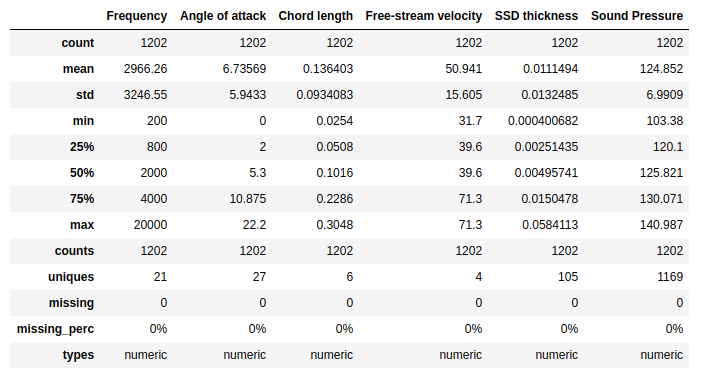
\includegraphics[scale=0.55]{img/train_summary.png}
\caption{Tabla que contiene el resumen de los datos de training.}
\end{figure}

    Aquí podemos ver que para ninguna de las variables faltan datos, lo cuál
nos ahorra tiempo extra de procesado en el que tendríamos que insertar
valores a partir de algún valor estadístico (valores medios, por
ejemplo).

También podemos ver información sobre como varían los datos, tanto los
de entrada como los de salida. Vemos que, por ejemplo,
\textbf{Frequency} es una característica que varía mucho, ya que tiene
unos valores mínimos y máximos muy dispares, además de tener una
desviación típica muy elevada. Posiblemente este atributo contenga
\emph{outliers}, pero al no disponer de demasiados datos, y al ser tan
pocos los posibles valores anómalos, no merece la pena intentar
eliminarlos. Observando el resto de características, nos encontramos con
unos valores que varían menos y cuyos rangos de valores más pequeño. Lo
sorprendente es que, para los datos de entrada, tenemos que hay muy
pocos valores únicos (no repetidos). Esto se puede deber a que no se han
medido los valores con suficiente precisión o a que no exista una
verdadera variabilidad entre ellos. Para los datos de salida, en cambio,
nos encontramos que hay un montón de valores distintos. Esto es normal,
ya que, al ser valores reales, hay muchos posibles valores. De aquí
podemos concluir que, a pesar de que nos encontremos ante un problema
con variable reales, parece que los valores que toman las variables de
entrada están discretizados, es decir, que no son exactamente contínuos.

Pasemos ahora a analizar el conjunto de datos de entrenamiento. Para
obtener suficiente información, vamos a fijarnos solo en valores únicos
y si faltan datos, teniendo en cuenta que nunca debemos obtener
información completa sobre los datos de test, ya que se supone que nunca
serán conocidos y que nunca deberíamos verlos. A continuación, podemos
ver esta información:

    \begin{Verbatim}[commandchars=\\\{\}]
{\color{incolor}In [{\color{incolor}5}]:} \PY{c+c1}{\PYZsh{} Crear DataFrame con los datos de test}
        \PY{n}{test\PYZus{}df} \PY{o}{=} \PY{n}{pd}\PY{o}{.}\PY{n}{DataFrame}\PY{p}{(}\PY{n}{columns}\PY{o}{=}\PY{n}{column\PYZus{}names}\PY{p}{,}
                               \PY{n}{data}\PY{o}{=}\PY{n}{np}\PY{o}{.}\PY{n}{c\PYZus{}}\PY{p}{[}\PY{n}{X\PYZus{}test}\PY{p}{,} \PY{n}{y\PYZus{}test}\PY{p}{]}\PY{p}{)}
        
        \PY{c+c1}{\PYZsh{} Crear un DataFrame resumen y mostrar algunos}
        \PY{c+c1}{\PYZsh{} valores estadísticos}
        \PY{n}{test\PYZus{}sum} \PY{o}{=} \PY{n}{DataFrameSummary}\PY{p}{(}\PY{n}{test\PYZus{}df}\PY{p}{)}\PY{o}{.}\PY{n}{columns\PYZus{}stats}
        \PY{n}{display}\PY{p}{(}\PY{n}{test\PYZus{}sum}\PY{p}{)}
\end{Verbatim}

\begin{figure}[H]
\centering
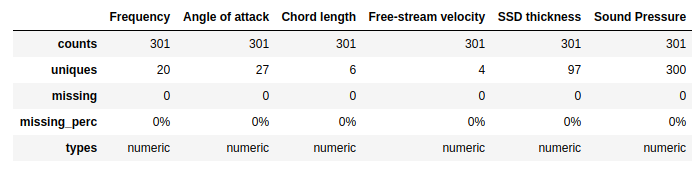
\includegraphics[scale=0.55]{img/test_summary.png}
\caption{Tabla que contiene el resumen de los datos de test.}
\end{figure}

Como se puede ver, el número de valores únicos, para las variables de
entrada, son muy próximos a los que teníamos anteriormente. En el caso
de los valores de salida, podemos observar que hay mucha diversidad. Y,
finalmente, como punto positivo, podemos ver que en ninguna de las
muestras faltan datos.

Una vez hecho este pequeño análisis, pasemos a observar ahora la
correlación entre las variables. Vamos a intentar obtener, para cada una
de las variables (tanto las de entrada como las de salida) el
coeficiente de correlación de Pearson. El resultado se puede ver a
continuación:

    \begin{Verbatim}[commandchars=\\\{\}]
{\color{incolor}In [{\color{incolor}6}]:} \PY{c+c1}{\PYZsh{} Obtener gráfica de correlación de Pearson}
        \PY{n}{corr} \PY{o}{=} \PY{n}{train\PYZus{}df}\PY{o}{.}\PY{n}{corr}\PY{p}{(}\PY{p}{)}
        \PY{n}{corr}\PY{o}{.}\PY{n}{style}\PY{o}{.}\PY{n}{background\PYZus{}gradient}\PY{p}{(}\PY{n}{cmap}\PY{o}{=}\PY{l+s+s1}{\PYZsq{}}\PY{l+s+s1}{Spectral}\PY{l+s+s1}{\PYZsq{}}\PY{p}{)}
\end{Verbatim}

\begin{figure}[H]
\centering
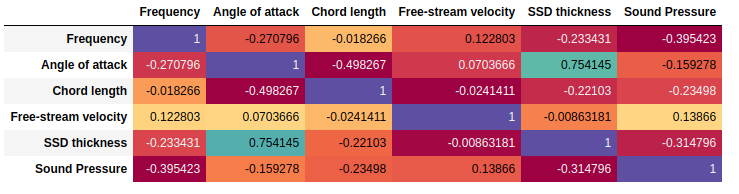
\includegraphics[scale=0.5]{img/tabla_correlacion.png}
\caption{Tabla con los coeficientes de Pearson para cada par de variables.}
\end{figure}
            
    Se puede ver que, en general, no existe una correlación entre la mayoría
de las características. Sin embargo, sí que destacan dos casos, uno más
que el otro. El primer caso es la relación que existe entre la
característica \textbf{SSD thickness} y la característica \textbf{Angle
of attack}. Estas dos características tienen una coeficiente de
correlación de Pearson de \(0.75\), valor que es muy próximo a \(1\).
Por tanto, podemos decir que existe cierta correlación entre ellas, ya
que el crecimiento de una influirá en el crecimiento de la otra. Sin
embargo, como el valor del coeficiente de Pearson no es 1, no podríamos
asegurar con absoluta confianza que las 2 características estén
correlacionadas, y que por tanto, sería necesario eliminar una de ellas.
El segundo caso es \textbf{Chord length} y \textbf{Angle of attack}.
Aquí lo que sucede es que el coeficiente de correlación de Pearson tiene
un valor de aproximadamente \(-0.5\). Con lo cuál, a pesar de que existe
cierta correlación negativa entre las dos variables (cuando crezca una,
la otra decrecerá), no podríamos afirmar con un 100\% de confianza que
estén totalmente correlacionadas, ya que el valor del coeficiente está
en un punto medio.

Para tener una mejor visión de todo lo que se acaba a discutir, vamos a
ver un conjunto de gráficas en las que se pueden ver los valores de
todas las variables dos a dos (es decir, se muestran gráficas para
mostrar como cambia cada par de variables, que pueden ser tanto las
características como la etiqueta de salida). Esto se puede ver a
continuación:

    \begin{Verbatim}[commandchars=\\\{\}]
{\color{incolor}In [{\color{incolor}7}]:} \PY{c+c1}{\PYZsh{} Módulo avanzado para dibujar gráficas}
        \PY{k+kn}{import} \PY{n+nn}{seaborn} \PY{k}{as} \PY{n+nn}{sns}
        
        \PY{c+c1}{\PYZsh{} Crear pares de plots para cada 2 atributos}
        \PY{c+c1}{\PYZsh{} También se incluyen las etiquetas}
        \PY{n}{sns}\PY{o}{.}\PY{n}{set\PYZus{}style}\PY{p}{(}\PY{l+s+s2}{\PYZdq{}}\PY{l+s+s2}{whitegrid}\PY{l+s+s2}{\PYZdq{}}\PY{p}{)}
        \PY{n}{sns}\PY{o}{.}\PY{n}{pairplot}\PY{p}{(}\PY{n}{train\PYZus{}df}\PY{p}{)}
        
        \PY{c+c1}{\PYZsh{} Mostrar el plot}
        \PY{n}{plt}\PY{o}{.}\PY{n}{show}\PY{p}{(}\PY{p}{)}
\end{Verbatim}

\begin{figure}[H]
\centering
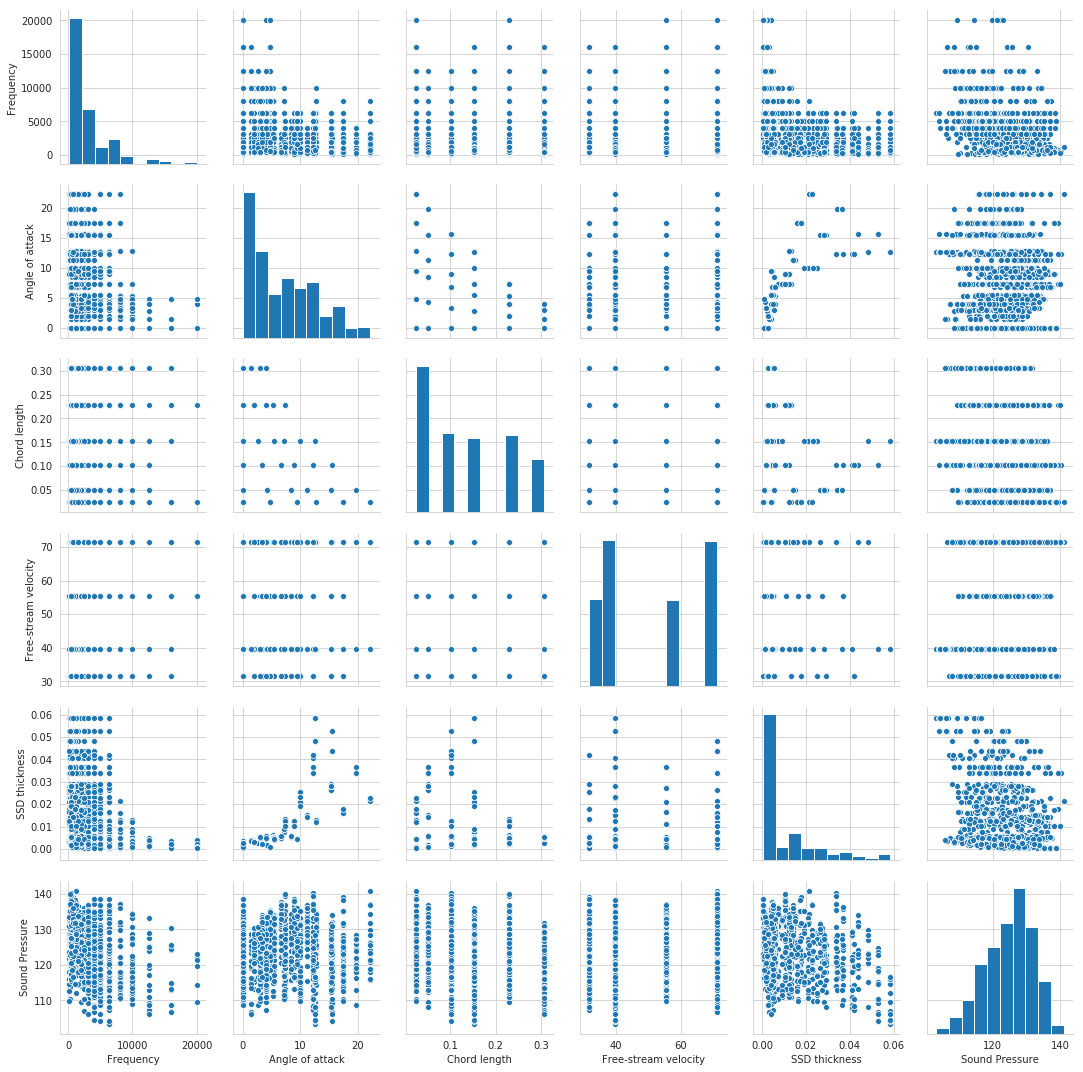
\includegraphics[scale=0.35]{img/output_17_0.png}
\caption{Gráficas que muestran como varían todas las variables dos a dos.}
\end{figure}

En estas gráficas se puede ver más claramente lo que se ha comentado
anteriormente. Se puede ver, por ejemplo, como entre \textbf{SSD
thickness} y \textbf{Angle of attack} existe cierta correlación, lo cuál
confirma nuestra hipótesis anterior. Se puede ver, por ejemplo, en el
gráfico en el que \textbf{SSD thickness} está en el eje \(Y\) y
\textbf{Angle of attack} en el \(X\). Se puede observar que, a medida
que va creciendo el valor de \textbf{SSD thickness}, parece que el otro
va creciendo como si fuese un polinomio de grado 2. Cambiando los ejes
de las variables, podemos ver que el crecimiento pasa a ser o bien
logarítmico o bien una raíz cuadrada.

Estudiando el caso de \textbf{Chord length} y \textbf{Angle of attack},
se puede ver que en los dos casos, a medida que se va incrementando el
valor de la variable situada en el eje \(X\), la que se encuentra en el
eje \(Y\) va disminuyendo de una forma que parece lineal.

Además, gracias a esta visualización hemos descubierto otra posbile
correlación entre 2 variables: la que puede existir entre \textbf{SSD
thickness} y \textbf{Frequency}. Aquí pasa algo muy parecido al caso
anterior. A medida que una va aumentando su valor en el eje \(X\), la
otra va disminuyendo su valor en el eje \(Y\) de una forma que nos
recuerda a un polinomio de grado 2. Esta correlación hubiese sido
difícil de ver solo con la tabla de correlaciones que teníamos
anteriormente, pero gracias a las gráficas se puede ver de una forma más
clara.

Para acabar este apartado de análisis, a pesar de haber descubierto que
pueden existir correlaciones entre algunas variables, de momento vamos a
decidir \textbf{no eliminar ninguna de las variables de entrada}, ya que
en este problema no tenemos muchas dimensiones y los datos provienen de
una fuente fiable como por ejemplo sería la NASA, así que supondremos
que han realizado un buen trabajo procesando los datos antes de hacerlos
públicos.

    \subsection{Selección de funciones}\label{selecciuxf3n-de-funciones}

    Antes de continuar con la elección de modelo, vamos a comentar algunos
aspectos a tener en cuenta, como por ejemplo qué funciones vamos a
utilizar.

Para este problema, dado que hay pocas dimensiones y con el objetivo de
intentar evitar un posible sobreajuste si se aplica alguna
transformación no lineal a los datos, vamos a utilizar alguna función
que sea \textbf{combinación lineal} de éstos, además de que son las
funciones más sencillas de probar a priori y se considera buena práctica
intentar utilizar estas funciones de primeras. Por tanto, nuestro
objetivo será encontrar una función \(g\) que, al realizar una
combinación lineal de los datos de entrada nos permita obtener un valor
real de salida. En caso de ver que nuestra función lineal nos ofrece un
E\(_{test}\) malo, podríamos intentar utilizar alguna transformación no
lineal, como por ejemplo añadir los cuadrados de las entradas, aunque en
un principio no se hará esto.

    \subsection{Selección de métricas}\label{selecciuxf3n-de-muxe9tricas}

    Otro aspecto que tenemos que comentar, antes de pasar a hablar de los
modelos a evaluar, es la métrica que utilizaremos tanto a la hora de
ajustar los distintos modelos como para evaluar los modelos y elegir el
mejor de ellos.

\subsubsection{Métrica del ajuste}\label{muxe9trica-del-ajuste}

Todos los modelos utilizarán la \emph{loss function} o métrica MSE (Mean
Squared Error, error cuadrático o norma \(\ell 2\)) cuando sean
ajustados. Esto se debe a que queremos penalizar más los errores que se
alejen más de los valores reales que aquellos que se alejen solo un
poco.

\subsubsection{Métrica de evaluación}\label{muxe9trica-de-evaluaciuxf3n}

Para evaluar los modelos, vamos a utilizar como métrica el MAE (Mean
Absolute Error, error absoluto o normal \(\ell 1\)). El motivo de esto
es que queremos ver cúanta variabilidad real hay en los valores
predichos, sin penalizar ningún tipo de error más que otro, además de
que es más fácilmente interpretable (se van acumulando todos los errores
en vez de acumular los cuadrados de éstos).

    \subsection{Selección de modelos a
evaluar}\label{selecciuxf3n-de-modelos-a-evaluar}

Finalmente, vamos a describir los modelos que se quieren evaluar para
poder elegir el mejor de ellos y el por qué de cada uno.

\subsubsection{Regresión lineal}\label{regresiuxf3n-lineal}

El primer modelo que queremos evaluar es la regresión lineal, sin ningún
tipo de regularización. Queremos evaluar su rendimiento respecto a
modelos que intentan ofrecer mejores resultados mediante regularización
o algo más complejos pero sin salir de los modelos lineales.

\subsubsection{\texorpdfstring{\emph{Ridge
Regression}}{Ridge Regression}}\label{ridge-regression}

El segundo modelo que queremos evaluar es la \emph{Ridge Regressión}, o
dicho de otra forma, regresión lineal con regularización de tipo norma
\(\ell 2\). Es decir, habría que resolver un problema de tipo:

\begin{equation}
\min_{w} || X w - y||_2^2 + \alpha ||w||_2^2
\end{equation}

Esta regularización, lo que hace, es añadir la suma de los cuadrados de
cada uno de los \(w_i \in w\), ponderada con un hiperparámetro
\(\alpha\) que se tiene que elegir.

El motivo por el que se ha escogido este modelo es porque se intenta
mejorar la regresión lineal, restringiendo el espacio de soluciones para
intentar evitar tanto el sobreajuste como resultados pobres. Es
importante decir que se ha preferido utilizar \emph{Ridge} como forma de
regularización sobre \emph{Lasso} (norma \(\ell 1\)) debido a que esta
última busca reducir el número de características ponderando cuantas más
pueda con un valor de \(0\), cosa que no nos interesa en este problema
ya que no disponemos de muchas variables.

\subsubsection{\texorpdfstring{SVM con \emph{kernel}
lineal}{SVM con kernel lineal}}\label{svm-con-kernel-lineal}

El último modelo que queremos evaluar es el SVM de regresión con
\emph{kernel} lineal, con el objetivo de ver si es capaz de ganarle a la
regresión lineal normal y a la \emph{Ridge Regression}. Esta es una
técnica más avanzada y un poco más compleja que el SVM utilizado en
clasificación, ya que aquí se tienen algunos parámetros más.

El objetivo aquí es intentar encontrar el mejor plano o uno muy bueno
dentro de un margen (debido a que en problemas de regresión hay
infinitos planos ya que hay infinitos valores reales) dado por el valor
de un \(\epsilon\), minimizando la suma de los valores de violación del
margen (aquellos puntos fuera del margen) dados por \(\xi_n\) para cada
punto de la muestra (lo contrario a lo que hace SVM en clasificación).
Cuanto más peso se le de a esta sumatoria mediante un valor \(C\), más
se ajustará el modelo, pero por tanto, habrán más probabilidades de que
se produzca \emph{overfitting}.

    \subsection{Elección del mejor
modelo}\label{elecciuxf3n-del-mejor-modelo}

Para elegir el mejor modelo, vamos a llevar a cabo un proceso que nos
permita comparar los modelos con los datos que tenemos. Para hacer esto,
la mejor manera de hacerlo es utilizar un \textbf{10-fold
cross-validation} con los datos de training. Es decir, se harán 10
particiones disjuntas de los datos, se entrenará el modelo con 9 de
ellas y se usará la última para validar el modelo. Esto se hará 10 veces
(cada vez una de las particiones será usada como partición de
validación), y se obtendrá un valor medio de E\(_{val}\) que nos
permitirá saber aproximadamente lo bueno que es el modelo utilizado.
Esto tiene un pequeño inconveniente, y es que perdemos datos que
utilizar en el entrenamiento de los modelos, con lo cuál los resultados
obtenidos posiblemente no sean los mejores. Sin embargo, es un pequeño
precio a pagar, ya que así podremos tener una estimación bastante buena
del posible error fuera de la muestra. Una vez escogido el mejor modelo,
se intentarán mejorar los hiperparámetros de éste para ver cuáles son
los mejores, y finalmente se entrenará con todo el conjunto de training.

Antes de comenzar con la elección, hay que tener en cuenta algo muy
importante. Ya que tenemos datos con escalas muy diversas y con
variabilidad diferente, vamos a tener que escalar los datos. Para hacer
eso, podemos, por ejemplo, restar a cada valor de cada característica la
media de esa característica y dividir este resultado entre la desviación
típica de esa característica. Con esto, conseguimos que los datos tengan
una distribución normal con \(\mu = 0\) y \(\sigma = 1\). Sin embargo,
esto no lo podemos aplicar sobre todo el conjunto de training hasta que
no tengamos el modelo definitivo elegido. El motivo es que, al hacer el
\textbf{10-fold cross-validation}, una parte de los datos será utilizada
para evaluar el modelo. Si todos los datos se han escalado antes de
realizar las particiones, se puede dar el caso de que los resultados que
se obtengan sean mejores de los que deberían ser. Además, estaríamos
modificando datos a los que en un principio no tendríamos acceso (como
por ejemplo los datos de test más adelante o los de evaluación en cada
fold). Por tanto, en cada fold lo que ser hará es que primero se
escalarán los datos con los que se entrena, después se entrenará el
modelo y después se escalarán los datos de evaluación y se obtendrán los
valores predichos. Un proceso similar será utilizado más adelante con
los datos de test, pero cuando llegue el momento ser recalcará de nuevo.
Y con esto dicho, comencemos con el proceso de elección del mejor
modelo.

Para cada modelo, vamos a ir probando un conjunto de hiperparámetros y
vamos a ver qué resultados obtenemos en cada caso. Por ejemplo, en
regresión lineal, no hay hiperparámetros que configurar, con lo cuál
será una prueba directa. En el caso de \emph{Ridge Regression} vamos a
probar con algunos valores de \(\alpha\), como por ejemplo \(0.2\),
\(0.5\) y \(1\) (regularización floja, de intensidad media y fuerte). En
el caso de SVM con \emph{kernel} lineal, los hiperparámetros con los que
probaremos serán \(\epsilon\) y \(C\), y probaremos con valores como
\(0.2\) y \(1\) para \(\epsilon\), y \(0.1\) y \(1\) para \(C\).

Para ayudarnos con este proceso, vamos a utilizar una funcionalidad que
nos permita agrupar un conjunto de operaciones en los que se transformen
los datos, se ajuste un modelo, se transformen los datos de evaluación y
se predigan los valores, y podamos obtener los valores estadísticos de
evaluación luego. Esta funcionalidad se llama ``\emph{pipeline}'', y puede
ser aplicada incluso con algún tipo de \textbf{k-fold}. Primero, vamos a
crear una serie de funciones que nos permitan obtener pipelines para
cada uno de los modelos a evaluar, con los hiperparámteros preparados.
Vamos a ver cuáles son estas funciones que se utilizan para crear los
\emph{pipelines} que usaremos luego:

 \begin{Verbatim}[commandchars=\\\{\}]
{\color{incolor}In [{\color{incolor}8}]:} \PY{c+c1}{\PYZsh{} Importar funcionalidades para crear pipelines}
        \PY{k+kn}{from} \PY{n+nn}{sklearn}\PY{n+nn}{.}\PY{n+nn}{pipeline} \PY{k}{import} \PY{n}{make\PYZus{}pipeline}
        \PY{k+kn}{from} \PY{n+nn}{sklearn}\PY{n+nn}{.}\PY{n+nn}{pipeline} \PY{k}{import} \PY{n}{Pipeline}
        
        \PY{c+c1}{\PYZsh{} Importar escalado de datos que se va a aplicar}
        \PY{k+kn}{from} \PY{n+nn}{sklearn}\PY{n+nn}{.}\PY{n+nn}{preprocessing} \PY{k}{import} \PY{n}{StandardScaler}
        
        \PY{c+c1}{\PYZsh{} Importar modelos que se van a utilizar}
        \PY{k+kn}{from} \PY{n+nn}{sklearn}\PY{n+nn}{.}\PY{n+nn}{linear\PYZus{}model} \PY{k}{import} \PY{n}{LinearRegression}\PY{p}{,} \PY{n}{Ridge}
        \PY{k+kn}{from} \PY{n+nn}{sklearn}\PY{n+nn}{.}\PY{n+nn}{svm} \PY{k}{import} \PY{n}{LinearSVR}
        
        \PY{c+c1}{\PYZsh{} Importar funcionalidad para probar pipelines}
        \PY{k+kn}{from} \PY{n+nn}{sklearn}\PY{n+nn}{.}\PY{n+nn}{model\PYZus{}selection} \PY{k}{import} \PY{n}{cross\PYZus{}val\PYZus{}score}
        
        \PY{k}{def} \PY{n+nf}{create\PYZus{}ridge\PYZus{}pipelines}\PY{p}{(}\PY{n}{alpha}\PY{p}{)}\PY{p}{:}
            \PY{l+s+sd}{\PYZdq{}\PYZdq{}\PYZdq{}}
        \PY{l+s+sd}{    Funcion para crear una lista de pipelines para Ridge}
        \PY{l+s+sd}{    Regression con un valor de alfa para cada uno}
        \PY{l+s+sd}{    }
        \PY{l+s+sd}{    :param alpha: Valor alfa asociado a la ponderacion de}
        \PY{l+s+sd}{                  la regularizacion}
        \PY{l+s+sd}{    }
        \PY{l+s+sd}{    :return Devuelve una lista de pipelines, cada uno con}
        \PY{l+s+sd}{            su propio valor de alfa}
        \PY{l+s+sd}{    \PYZdq{}\PYZdq{}\PYZdq{}}
            
            \PY{c+c1}{\PYZsh{} Creamos una nueva lista de pipelines}
            \PY{n}{pipelines} \PY{o}{=} \PY{p}{[}\PY{p}{]}
            
            \PY{c+c1}{\PYZsh{} Insertamos un nuevo pipeline que utiliza StandardScaler}
            \PY{c+c1}{\PYZsh{} y Ridge Regression con un valor de alpha dado}
            \PY{k}{for} \PY{n}{a} \PY{o+ow}{in} \PY{n}{alpha}\PY{p}{:}
                \PY{n}{pipelines}\PY{o}{.}\PY{n}{append}\PY{p}{(}\PY{n}{make\PYZus{}pipeline}\PY{p}{(}\PY{n}{StandardScaler}\PY{p}{(}\PY{p}{)}\PY{p}{,}
                				\PY{n}{Ridge}\PY{p}{(}\PY{n}{alpha}\PY{o}{=}\PY{n}{a}\PY{p}{)}\PY{p}{)}\PY{p}{)}
            
            \PY{k}{return} \PY{n}{pipelines}
        
        
        \PY{k}{def} \PY{n+nf}{create\PYZus{}svmr\PYZus{}pipelines}\PY{p}{(}\PY{n}{epsilon}\PY{p}{,} \PY{n}{c\PYZus{}list}\PY{p}{)}\PY{p}{:}
            \PY{l+s+sd}{\PYZdq{}\PYZdq{}\PYZdq{}}
        \PY{l+s+sd}{    Funcion para crear una lista de pipelines para SVM}
        \PY{l+s+sd}{    Regression con una pareja de epsilon y C para cada}
        \PY{l+s+sd}{    uno.}
        \PY{l+s+sd}{    Cada elemento contiene un StandardScaler y un LinearSVR,}
        \PY{l+s+sd}{    que utilizara la norma l2 para el error, }
        \PY{l+s+sd}{    }
        \PY{l+s+sd}{    :param epsilon: Lista de valores epsilon asociados}
        \PY{l+s+sd}{                    a la amplitud del margen}
        \PY{l+s+sd}{    :param c\PYZus{}list: Lista de valores C que ponderan el error}
        \PY{l+s+sd}{    }
        \PY{l+s+sd}{    :return Devuelve una lista de pipelines, cada uno con}
        \PY{l+s+sd}{            sus propios epsilon y c}
        \PY{l+s+sd}{    \PYZdq{}\PYZdq{}\PYZdq{}}
            
            \PY{c+c1}{\PYZsh{} Crear una nueva lista de pipelines}
            \PY{n}{pipelines} \PY{o}{=} \PY{p}{[}\PY{p}{]}
            
            \PY{c+c1}{\PYZsh{} Insertar un nuevo pipeline que utiliza StandardScaler}
            \PY{c+c1}{\PYZsh{} y LinearSVR con los valors de epsilon y C dados en las}
            \PY{c+c1}{\PYZsh{} listas}
            \PY{k}{for} \PY{n}{e} \PY{o+ow}{in} \PY{n}{epsilon}\PY{p}{:}
                \PY{k}{for} \PY{n}{c} \PY{o+ow}{in} \PY{n}{c\PYZus{}list}\PY{p}{:}
                    \PY{n}{pipelines}\PY{o}{.}\PY{n}{append}\PY{p}{(}\PY{n}{make\PYZus{}pipeline}\PY{p}{(}\PY{n}{StandardScaler}\PY{p}{(}\PY{p}{)}\PY{p}{,}
                        \PY{n}{LinearSVR}\PY{p}{(}\PY{n}{epsilon}\PY{o}{=}\PY{n}{e}\PY{p}{,} \PY{n}{C}\PY{o}{=}\PY{n}{c}\PY{p}{,} \PY{n}{random\PYZus{}state}\PY{o}{=}\PY{l+m+mi}{1}
				\PY{n}{loss}\PY{o}{=}\PY{l+s+s1}{\PYZsq{}}\PY{l+s+s1}{squared\PYZus{}epsilon\PYZus{}insensitive}\PY{l+s+s1}{\PYZsq{}}\PY{p}{)}\PY{p}{)}\PY{p}{)}
            
            \PY{k}{return} \PY{n}{pipelines}
\end{Verbatim}

 Una vez hecho esto, vamos a crear una función para evaluar los modelos.
Esta función se encargará de evaluar cada uno de los modelos que se le
pasen junto con los conjuntos de datos mediante la técnica del
\textbf{10-fold cross validation}. Irá guardando los valores medios de
los errores junto con su desviación típica. Con esta información,
podremos luego elegir el mejor modelo para este problema. La función que
se encarga de realizar la evaluación individual de cada modelo se
encargará de aplicar todas las operaciones que se le especifiquen
automáticamente, sin tener que preocuparnos nostros. Todo esto se puede
ver en el siguiente código:

    \begin{Verbatim}[commandchars=\\\{\}]
{\color{incolor}In [{\color{incolor}9}]:} \PY{k}{def} \PY{n+nf}{evaluate\PYZus{}models}\PY{p}{(}\PY{n}{models}\PY{p}{,} \PY{n}{X}\PY{p}{,} \PY{n}{y}\PY{p}{,} \PY{n}{cv}\PY{o}{=}\PY{l+m+mi}{10}\PY{p}{,}
			    \PY{n}{metric}\PY{o}{=}\PY{l+s+s1}{\PYZsq{}}\PY{l+s+s1}{neg\PYZus{}mean\PYZus{}absolute\PYZus{}error}\PY{l+s+s1}{\PYZsq{}}\PY{p}{)}\PY{p}{:}
            \PY{l+s+sd}{\PYZdq{}\PYZdq{}\PYZdq{}}
        \PY{l+s+sd}{    Funcion para evaluar un conjunto de modelos con un conjunto}
        \PY{l+s+sd}{    de caracteristicas y etiquetas.}
        \PY{l+s+sd}{    }
        \PY{l+s+sd}{    }
        \PY{l+s+sd}{    :param models: Lista que contiene pipelines o modelos que}
        \PY{l+s+sd}{                   se quieren evaluar}
        \PY{l+s+sd}{    :param X: Conjunto de datos con los que evaluar}
        \PY{l+s+sd}{    :param y: Conjunto de etiquetas}
        \PY{l+s+sd}{    :param cv: Numero de k\PYZhy{}folds que realizar (por defecto 10)}
        \PY{l+s+sd}{    :param metric: Metrica de evaluacion (por defecto es la}
        \PY{l+s+sd}{                    norma\PYZhy{}l1, neg\PYZus{}mean\PYZus{}absolute\PYZus{}error)}
        \PY{l+s+sd}{    }
        \PY{l+s+sd}{    :return Devuelve una lista con los valores medios y una}
        \PY{l+s+sd}{            lista con las desviaciones tipicas}
        \PY{l+s+sd}{    \PYZdq{}\PYZdq{}\PYZdq{}}
            
            \PY{c+c1}{\PYZsh{} Crear listas de medias y desviaciones}
            \PY{n}{means} \PY{o}{=} \PY{p}{[}\PY{p}{]}
            \PY{n}{deviations} \PY{o}{=} \PY{p}{[}\PY{p}{]}
            
            \PY{c+c1}{\PYZsh{} Para cada modelo, obtener los resultados de}
            \PY{c+c1}{\PYZsh{} evaluar el modelo con todas las particiones}
            \PY{c+c1}{\PYZsh{} Guardar los resultados en las listas correspondientes}
            \PY{k}{for} \PY{n}{model} \PY{o+ow}{in} \PY{n}{models}\PY{p}{:}
                \PY{n}{results} \PY{o}{=} \PY{n}{cross\PYZus{}val\PYZus{}score}\PY{p}{(}\PY{n}{model}\PY{p}{,} \PY{n}{X}\PY{p}{,} \PY{n}{y}\PY{p}{,} \PY{n}{scoring}\PY{o}{=}\PY{n}{metric}\PY{p}{,}
                			  \PY{n}{cv}\PY{o}{=}\PY{n}{cv}\PY{p}{)}
                
                \PY{c+c1}{\PYZsh{} Guardar valor medio de los errores}
                \PY{c+c1}{\PYZsh{} Se guarda el valor absoluto porque son valores}
                \PY{c+c1}{\PYZsh{} negativos}
                \PY{n}{means}\PY{o}{.}\PY{n}{append}\PY{p}{(}\PY{n+nb}{abs}\PY{p}{(}\PY{n}{results}\PY{o}{.}\PY{n}{mean}\PY{p}{(}\PY{p}{)}\PY{p}{)}\PY{p}{)}
                
                \PY{c+c1}{\PYZsh{} Guardar desviaciones}
                \PY{n}{deviations}\PY{o}{.}\PY{n}{append}\PY{p}{(}\PY{n}{np}\PY{o}{.}\PY{n}{std}\PY{p}{(}\PY{n}{results}\PY{p}{)}\PY{p}{)}
            
            \PY{k}{return} \PY{n}{means}\PY{p}{,} \PY{n}{deviations}
\end{Verbatim}

    Con esto, ya podemos evaluar los modelos que hemos propuesto
anteriormente y ver cuál sería el mejor. Pero antes, vamos a crear una
función que nos permita visualizar la informacion referente a los
resultados de evaluar los distintos modelos:

\begin{Verbatim}[commandchars=\\\{\}]
{\color{incolor}In [{\color{incolor}10}]:} \PY{k}{def} \PY{n+nf}{print\PYZus{}evaluation\PYZus{}results}\PY{p}{(}\PY{n}{models}\PY{p}{,} \PY{n}{means}\PY{p}{,} \PY{n}{deviations}\PY{p}{,}
				      \PY{n}{metric}\PY{p}{)}\PY{p}{:}
             \PY{l+s+sd}{\PYZdq{}\PYZdq{}\PYZdq{}}
         \PY{l+s+sd}{    Funcion para mostrar por pantalla los resultados}
         \PY{l+s+sd}{    de la evaluacion}
         \PY{l+s+sd}{    }
         \PY{l+s+sd}{    :param models: Nombres de los modelos evaluados}
         \PY{l+s+sd}{    :param means: Lista con los valores medios de las}
         \PY{l+s+sd}{                  evaluaciones}
         \PY{l+s+sd}{    :param deviations: Lista con los valores de las}
         \PY{l+s+sd}{                       desv. tipicas de las evaluaciones}
         \PY{l+s+sd}{    :param metric: Metrica a evaluar}
         \PY{l+s+sd}{    \PYZdq{}\PYZdq{}\PYZdq{}}
             
             \PY{n+nb}{print}\PY{p}{(}\PY{l+s+s1}{\PYZsq{}}\PY{l+s+s1}{Evaluation results for each model}\PY{l+s+s1}{\PYZsq{}}\PY{p}{)}
             
             \PY{c+c1}{\PYZsh{} Crear un DataFrame con el formato de salida}
             \PY{n}{out\PYZus{}df} \PY{o}{=} \PY{n}{pd}\PY{o}{.}\PY{n}{DataFrame}\PY{p}{(}\PY{n}{index}\PY{o}{=}\PY{n}{models}\PY{p}{,}
               \PY{n}{columns}\PY{o}{=}\PY{p}{[}\PY{n}{metric}\PY{p}{,} \PY{l+s+s1}{\PYZsq{}}\PY{l+s+s1}{Standard Deviation}\PY{l+s+s1}{\PYZsq{}}\PY{p}{]}\PY{p}{,}
               \PY{n}{data}\PY{o}{=}\PY{p}{[}\PY{p}{[}\PY{n}{mean}\PY{p}{,} \PY{n}{dev}\PY{p}{]} \PY{k}{for} \PY{n}{mean}\PY{p}{,} \PY{n}{dev} \PY{o+ow}{in} \PY{n+nb}{zip}\PY{p}{(}\PY{n}{means}\PY{p}{,} \PY{n}{deviations}\PY{p}{)}\PY{p}{]}\PY{p}{)}
             \PY{n}{display}\PY{p}{(}\PY{n}{out\PYZus{}df}\PY{p}{)}
\end{Verbatim}

    Vamos a crear ahora los modelos que queremos evaluar con los
hiperparámetros que hemos especificado anteriormente.

    \begin{Verbatim}[commandchars=\\\{\}]
{\color{incolor}In [{\color{incolor}11}]:} \PY{c+c1}{\PYZsh{} Crear listas con hiperparametros para Ridge}
         \PY{n}{ridge\PYZus{}alpha} \PY{o}{=} \PY{p}{[}\PY{l+m+mf}{0.2}\PY{p}{,} \PY{l+m+mf}{0.5}\PY{p}{,} \PY{l+m+mf}{1.0}\PY{p}{]}
         
         \PY{c+c1}{\PYZsh{} Crear listas con hiperparametros para SVR}
         \PY{n}{svmr\PYZus{}epsilon} \PY{o}{=} \PY{p}{[}\PY{l+m+mf}{0.2}\PY{p}{,} \PY{l+m+mf}{1.5}\PY{p}{]}
         \PY{n}{svmr\PYZus{}c} \PY{o}{=} \PY{p}{[}\PY{l+m+mf}{0.1}\PY{p}{,} \PY{l+m+mf}{1.0}\PY{p}{]}
         
         \PY{c+c1}{\PYZsh{} Crear los nombres de los modelos}
         \PY{n}{model\PYZus{}names} \PY{o}{=} \PY{p}{[}\PY{l+s+s1}{\PYZsq{}}\PY{l+s+s1}{Linear Regression}\PY{l+s+s1}{\PYZsq{}}\PY{p}{,} \PY{l+s+s1}{\PYZsq{}}\PY{l+s+s1}{Ridge alpha=0.2}\PY{l+s+s1}{\PYZsq{}}\PY{p}{,}
                        \PY{l+s+s1}{\PYZsq{}}\PY{l+s+s1}{Ridge alpha=0.5}\PY{l+s+s1}{\PYZsq{}}\PY{p}{,} \PY{l+s+s1}{\PYZsq{}}\PY{l+s+s1}{Ridge alpha=1.0}\PY{l+s+s1}{\PYZsq{}}\PY{p}{,}
                        \PY{l+s+s1}{\PYZsq{}}\PY{l+s+s1}{SVMR e=0.2, c=0.1}\PY{l+s+s1}{\PYZsq{}}\PY{p}{,} \PY{l+s+s1}{\PYZsq{}}\PY{l+s+s1}{SVMR e=0.2, c=1.0}\PY{l+s+s1}{\PYZsq{}}\PY{p}{,}
                        \PY{l+s+s1}{\PYZsq{}}\PY{l+s+s1}{SVMR e=1.0, c=0.1}\PY{l+s+s1}{\PYZsq{}}\PY{p}{,} \PY{l+s+s1}{\PYZsq{}}\PY{l+s+s1}{SVMR e=1.0, c=1.0}\PY{l+s+s1}{\PYZsq{}}\PY{p}{]}
         
         \PY{c+c1}{\PYZsh{} Crear pipelines para cada modelo}
         \PY{n}{reg\PYZus{}pipe} \PY{o}{=} \PY{p}{[}\PY{n}{make\PYZus{}pipeline}\PY{p}{(}\PY{n}{StandardScaler}\PY{p}{(}\PY{p}{)}\PY{p}{,} \PY{n}{LinearRegression}\PY{p}{(}\PY{p}{)}\PY{p}{)}\PY{p}{]}
         \PY{n}{ridge\PYZus{}pipe} \PY{o}{=} \PY{n}{create\PYZus{}ridge\PYZus{}pipelines}\PY{p}{(}\PY{n}{ridge\PYZus{}alpha}\PY{p}{)}
         \PY{n}{svmr\PYZus{}pipe} \PY{o}{=} \PY{n}{create\PYZus{}svmr\PYZus{}pipelines}\PY{p}{(}\PY{n}{svmr\PYZus{}epsilon}\PY{p}{,} \PY{n}{svmr\PYZus{}c}\PY{p}{)}
         
         \PY{c+c1}{\PYZsh{} Juntar todos los pipelines en una lista con los modelos}
         \PY{n}{models} \PY{o}{=} \PY{n}{reg\PYZus{}pipe} \PY{o}{+} \PY{n}{ridge\PYZus{}pipe} \PY{o}{+} \PY{n}{svmr\PYZus{}pipe}
\end{Verbatim}

    Una vez preparados los modelos para ser evaluados, vamos a obtener los
valores estadísticos que nos permitan decidir cuál de ellos es el más
adecuado para este problema. El resultado se puede ver a continuación:

    \begin{Verbatim}[commandchars=\\\{\}]
{\color{incolor}In [{\color{incolor}12}]:} \PY{c+c1}{\PYZsh{} Obtener valores medios y desviaciones de las evaluaciones}
         \PY{n}{means}\PY{p}{,} \PY{n}{deviations} \PY{o}{=} \PY{n}{evaluate\PYZus{}models}\PY{p}{(}\PY{n}{models}\PY{p}{,} \PY{n}{X\PYZus{}train}\PY{p}{,} \PY{n}{y\PYZus{}train}\PY{p}{)}
         
         \PY{c+c1}{\PYZsh{} Mostrar valores por pantalla}
         \PY{n}{print\PYZus{}evaluation\PYZus{}results}\PY{p}{(}\PY{n}{model\PYZus{}names}\PY{p}{,} \PY{n}{means}\PY{p}{,} \PY{n}{deviations}\PY{p}{,}
         			 \PY{l+s+s1}{\PYZsq{}}\PY{l+s+s1}{Mean MAE}\PY{l+s+s1}{\PYZsq{}}\PY{p}{)}
\end{Verbatim}

    \begin{Verbatim}[commandchars=\\\{\}]
Evaluation results for each model

    \end{Verbatim}

\begin{figure}[H]
\centering
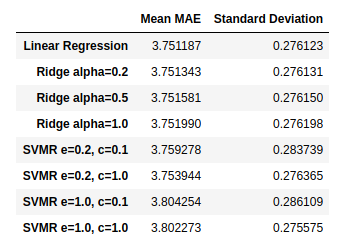
\includegraphics[scale=0.7]{img/evaluations_regression.png}
\end{figure}

A vista de los resultados obtenidos podemos extraer una serie de
conclusiones. En este caso, la Regresión Lineal sin ningún tipo de
regularización ha permitido obtener unos mejores resultados que
cualquiera de las otras técnicas. Ha conseguido el menor error medio de
entre todos ellos y es el segundo con menor desviación típica en los
resultados, con lo cuál se puede afirmar que los valores de los errores
para cada fold no variaban mucho. La \emph{Ridge Regression} ha
conseguido unos resultados buenos en general, ya que no dista mucho los
obtenidos por la Regresión Lineal. Los valores de los errores medios son
un poco peores y la desviación típica sube un poco comparada con la de
Regresión lineal, aunque a pesar de eso son unos resultados muy buenos.
SVM con \emph{kernel} lineal quedaría en último lugar, lo cuál no
indicaría que los resultados son del todo malos (con \(\epsilon = 0.2\)
parece acercarse a la Regresión Lineal). Es el modelo en el que más
varían los resultados de los errores y de las desviaciones, posiblemente
debido a los hiperparámetros. Al tener dos hiperparámetros que tiran
cada uno por un lado es difícil intentar ajustarlos correctamente a mano
para poder hacer pruebas satisfactorias. Posiblemente intentando ver
mejor como ajustar cada hiperparámetro se podrían haber conseguido unos
mejores resultados. A pesar de eso, a partir de los resultados podemos
afirmar que, para este problema, es preferible trabajar con valores de
\(\epsilon\) pequeños (son los que mejores resultados han permitido
obtener dentro del modelo SVM) e ir variando el valor de \(C\) hasta
encontrar un valor óptimo que permita obtener el menor error medio.

Como conlusión de aquí, podemos conluir que nuestro modelo definitivo es
la \textbf{Regresión Lineal}, y es la que vamos a ajusta a continuación.

    \subsection{Ajuste del modelo
seleccionado}\label{ajuste-del-modelo-seleccionado}

Una vez elegida la Regresión Lineal como nuestro modelo, vamos a
proceder a entrenar el modelo. Lo primero que tenemos que hacer es
escalar los datos, ya que tienen unos valores muy dispares y nos
interesaría que todos ellos tuviesen unos valores bastante próximos.
Esto lo haremos con la clase \emph{StandardScaler}, como hemos visto
anteriormente, que se encarga de restar la media y de dividir entre la
desviación típica para hacer que los datos tengan una distribución tal
que \(\mu = 0\) y \(\sigma = 1\). Esto se puede ver en el siguiente
código:

    \begin{Verbatim}[commandchars=\\\{\}]
{\color{incolor}In [{\color{incolor}13}]:} \PY{c+c1}{\PYZsh{} Creamos el objeto que vamos a usar para escalar}
         \PY{n}{scaler} \PY{o}{=} \PY{n}{StandardScaler}\PY{p}{(}\PY{p}{)}
         
         \PY{c+c1}{\PYZsh{} Ajustar el scaler y transformamos los datos}
         \PY{n}{scaler}\PY{o}{.}\PY{n}{fit}\PY{p}{(}\PY{n}{X\PYZus{}train}\PY{p}{)}
         \PY{n}{X\PYZus{}train} \PY{o}{=} \PY{n}{scaler}\PY{o}{.}\PY{n}{transform}\PY{p}{(}\PY{n}{X\PYZus{}train}\PY{p}{)}
\end{Verbatim}

    A continuación lo que tenemos que hacer es ajusta el modelo. Para ello,
vamos a crear un objeto de la clase \emph{LinearRegression} y vamos a
entrenarlo con los datos transformados anteriormente. El siguiente
código refleja lo que se queire hacer:

    \begin{Verbatim}[commandchars=\\\{\}]
{\color{incolor}In [{\color{incolor}14}]:} \PY{c+c1}{\PYZsh{} Creamos el modelo que vamos a ajusat}
         \PY{n}{reg} \PY{o}{=} \PY{n}{LinearRegression}\PY{p}{(}\PY{p}{)}
         
         \PY{c+c1}{\PYZsh{} Ajustar el modelo}
         \PY{n}{reg}\PY{o}{.}\PY{n}{fit}\PY{p}{(}\PY{n}{X\PYZus{}train}\PY{p}{,} \PY{n}{y\PYZus{}train}\PY{p}{)}
\end{Verbatim}

\subsection{\texorpdfstring{Estimación de
E\(_{out}\)}{Estimación de E\_\{out\}}}\label{estimaciuxf3n-de-e_out}

En este apartado vamos a estimar el valor de E\(_{out}\). Para hacerlo,
vamos a obtener el valor de E\(_{test}\) a partir del conjunto de test.
Sabemos que este valor es una buena estimación de E\(_{out}\), ya que
estamos usando datos de los cuáles no sabemos nada (los separamos de
training antes de comenzar con todo el proceso). Por tanto, es lo más
cercano que tenemos a obtener una medida del error fuera de la muestra.

Para ver como de bueno es el modelo elegido, vamos a compararlo con un
modelo de regresión medio. Este modelo se ajusta con el conjunto de
etiquetas de entrenamiento y predice todas las nuevas etiquetas con el
valor medio de las etiquetas con las que ha sido entrenado. Un ejemplo
de este modelo sería lo siguiente:

    \begin{Verbatim}[commandchars=\\\{\}]
{\color{incolor}In [{\color{incolor}15}]:} \PY{c+c1}{\PYZsh{} Clase del modelo de regresion medio}
         \PY{k}{class} \PY{n+nc}{MeanRegression}\PY{p}{:}
             \PY{k}{def} \PY{n+nf}{\PYZus{}\PYZus{}init\PYZus{}\PYZus{}}\PY{p}{(}\PY{n+nb+bp}{self}\PY{p}{)}\PY{p}{:}
                 \PY{n+nb+bp}{self}\PY{o}{.}\PY{n}{predict\PYZus{}value} \PY{o}{=} \PY{l+m+mi}{0}
                 
             \PY{k}{def} \PY{n+nf}{fit}\PY{p}{(}\PY{n+nb+bp}{self}\PY{p}{,} \PY{n}{y}\PY{p}{)}\PY{p}{:}
                 \PY{c+c1}{\PYZsh{} Calcular valor medio}
                 \PY{n+nb+bp}{self}\PY{o}{.}\PY{n}{predict\PYZus{}value} \PY{o}{=} \PY{n}{y}\PY{o}{.}\PY{n}{mean}\PY{p}{(}\PY{p}{)}
             
             \PY{k}{def} \PY{n+nf}{predict}\PY{p}{(}\PY{n+nb+bp}{self}\PY{p}{,} \PY{n}{y}\PY{p}{)}\PY{p}{:}
                 \PY{c+c1}{\PYZsh{} Crear array de predicted con el mismo tamaño que}
                 \PY{c+c1}{\PYZsh{} las etiquetas que se quieren predecir}
                 \PY{n}{predicted} \PY{o}{=} \PY{n}{np}\PY{o}{.}\PY{n}{full\PYZus{}like}\PY{p}{(}\PY{n}{y}\PY{p}{,} \PY{n+nb+bp}{self}\PY{o}{.}\PY{n}{predict\PYZus{}value}\PY{p}{)}
                 
                 \PY{k}{return} \PY{n}{predicted}
\end{Verbatim}

    Con esto, vamos a ver cuál sería el valor de los MAE para cada uno de
los modelos. Es necesario recordar que tenemos que escalar los datos de
test con los mismos valores con los que hemos escalado los datos de
training. Todo esto se puede ver a continuación:

    \begin{Verbatim}[commandchars=\\\{\}]
{\color{incolor}In [{\color{incolor}16}]:} \PY{c+c1}{\PYZsh{} Metrica MAE}
         \PY{k+kn}{from} \PY{n+nn}{sklearn}\PY{n+nn}{.}\PY{n+nn}{metrics} \PY{k}{import} \PY{n}{mean\PYZus{}absolute\PYZus{}error}
         
         \PY{c+c1}{\PYZsh{} Crear modelo de regresion media y ajustarlo}
         \PY{n}{mean\PYZus{}reg} \PY{o}{=} \PY{n}{MeanRegression}\PY{p}{(}\PY{p}{)}
         \PY{n}{mean\PYZus{}reg}\PY{o}{.}\PY{n}{fit}\PY{p}{(}\PY{n}{y\PYZus{}train}\PY{p}{)}
         
         \PY{c+c1}{\PYZsh{} Escalar datos de test}
         \PY{n}{X\PYZus{}test\PYZus{}transf} \PY{o}{=} \PY{n}{scaler}\PY{o}{.}\PY{n}{transform}\PY{p}{(}\PY{n}{X\PYZus{}test}\PY{p}{)}
         
         \PY{c+c1}{\PYZsh{} Predecir valores con cada modelo}
         \PY{n}{predict\PYZus{}reg} \PY{o}{=} \PY{n}{reg}\PY{o}{.}\PY{n}{predict}\PY{p}{(}\PY{n}{X\PYZus{}test\PYZus{}transf}\PY{p}{)}
         \PY{n}{predict\PYZus{}mean\PYZus{}reg} \PY{o}{=} \PY{n}{mean\PYZus{}reg}\PY{o}{.}\PY{n}{predict}\PY{p}{(}\PY{n}{y\PYZus{}test}\PY{p}{)}
         
         \PY{n}{reg\PYZus{}test\PYZus{}err} \PY{o}{=} \PY{n}{mean\PYZus{}absolute\PYZus{}error}\PY{p}{(}\PY{n}{y\PYZus{}test}\PY{p}{,} \PY{n}{predict\PYZus{}reg}\PY{p}{)}
         \PY{n}{mean\PYZus{}reg\PYZus{}test\PYZus{}err} \PY{o}{=} \PY{n}{mean\PYZus{}absolute\PYZus{}error}\PY{p}{(}\PY{n}{y\PYZus{}test}\PY{p}{,} \PY{n}{predict\PYZus{}mean\PYZus{}reg}\PY{p}{)}
         
         \PY{n+nb}{print}\PY{p}{(}\PY{l+s+s1}{\PYZsq{}}\PY{l+s+s1}{Linear Regression E\PYZus{}test = }\PY{l+s+s1}{\PYZsq{}}\PY{p}{,} \PY{n}{reg\PYZus{}test\PYZus{}err}\PY{p}{)}
         \PY{n+nb}{print}\PY{p}{(}\PY{l+s+s1}{\PYZsq{}}\PY{l+s+s1}{Mean Linear Regression E\PYZus{}test = }\PY{l+s+s1}{\PYZsq{}}\PY{p}{,} \PY{n}{mean\PYZus{}reg\PYZus{}test\PYZus{}err}\PY{p}{)}
         \PY{n+nb}{print}\PY{p}{(}\PY{l+s+s1}{\PYZsq{}}\PY{l+s+s1}{Error proportion MER / LR: }\PY{l+s+s1}{\PYZsq{}}\PY{p}{,}
                \PY{n}{mean\PYZus{}reg\PYZus{}test\PYZus{}err} \PY{o}{/} \PY{n}{reg\PYZus{}test\PYZus{}err}\PY{p}{)}
\end{Verbatim}

    \begin{Verbatim}[commandchars=\\\{\}]
Linear Regression E\_test =  3.728952169124226
Mean Linear Regression E\_test =  5.258650496680505
Error proportion MER / LR:  1.4102220297225054

    \end{Verbatim}

 Como se puede ver a partir de los resultados obtenidos, el valor de
E\(_{test}\) obtenido con el modelo de Regresión Lineal es muy bueno.
Este valor nuevo es incluso mejor que el que habíamos estimado antes con
el valor medio de E\(_{val}\) (recordemos que cuando estabamos evaluando
nuestros modelos obtuvimos para cada uno un error MAE medio, el cuál se
corresponde con E\(_{val}\)). Uno de los motivos principales por los que
se ha visto reducido el error es que ahora hemos ajustado el modelo con
todos los datos de training de los que disponíamos, en vez de con solo
una parte como sucedía en \textbf{cross validation}. Por tanto, a medida
que vayamos aumentando los datos de training, mejor ajuste obtendremos.
Con este valor de E\(_{test}\) podemos afirmar que el valor de
E\(_{out}\) será, a lo sumo, tan grande como E\(_{test}\). Es decir,
podemos afirmar que:

\begin{equation}
    \text{E}_{out} \leq \text{E}_{test}
\end{equation}

Pasando a analizar ahora el E\(_{test}\) obtenido por el modelo lineal
medio vemos que este error es mucho más elevado que el de Regresión
Lineal y que cualquiera de los modelos que hemos evaluado anteriormente.
Esto es porque como tal, el modelo no intenta predecir el valor de las
nuevas etiquetas, si no que, para cada nuevo dato que le llega, predice
que su etiqueta será la media de las etiquetas con las que ha sido
entrenado. Este enfoque es \emph{naive}, ya que nada asegura que la
muestra con la que ha sido ajustado representa lo suficientemente bien a
la población y que la desviación típica de los datos de la muestra sea
pequeña (los datos pueden variar mucho, y por tanto, la media no será un
buen estimador/predictor de nuevos datos).

Comparando este enfoque \emph{naive} con nuestro modelo seleccionado,
vemos que si pasamos de utilizar un modelo lineal medio a un modelo de
Regresión Lineal obtenemos una ganancia de \(1.41\), lo cuál significa
que el error del modelo lineal medio tiene un error que es \(1.41\)
veces mayor que el error de la Regresión Lineal. Por tanto, está claro
que de entre los dos nos quedaríamos con aquél que nos ofrece menor
error.

Para ver como de bien predice nuestro modelo los datos, vamos a ver una
gráfica en la que en el eje \(X\) se tendrán los valores reales de las
etiquetas y en el eje \(Y\) se tendrán los valores predichos:

    \begin{Verbatim}[commandchars=\\\{\}]
{\color{incolor}In [{\color{incolor}17}]:} \PY{c+c1}{\PYZsh{} Visualizar grafica comparativa de valores}
         \PY{c+c1}{\PYZsh{} Se comparan los valores reales y los predichos}
         \PY{n}{sns}\PY{o}{.}\PY{n}{scatterplot}\PY{p}{(}\PY{n}{x}\PY{o}{=}\PY{n}{y\PYZus{}test}\PY{p}{,} \PY{n}{y}\PY{o}{=}\PY{n}{predict\PYZus{}reg}\PY{p}{)}
         \PY{n}{plt}\PY{o}{.}\PY{n}{xlabel}\PY{p}{(}\PY{l+s+s1}{\PYZsq{}}\PY{l+s+s1}{Real values}\PY{l+s+s1}{\PYZsq{}}\PY{p}{)}
         \PY{n}{plt}\PY{o}{.}\PY{n}{ylabel}\PY{p}{(}\PY{l+s+s1}{\PYZsq{}}\PY{l+s+s1}{Predicted values}\PY{l+s+s1}{\PYZsq{}}\PY{p}{)}
         \PY{n}{plt}\PY{o}{.}\PY{n}{title}\PY{p}{(}\PY{l+s+s1}{\PYZsq{}}\PY{l+s+s1}{Difference between real and predicted values}\PY{l+s+s1}{\PYZsq{}}\PY{p}{)}
         \PY{n}{plt}\PY{o}{.}\PY{n}{show}\PY{p}{(}\PY{p}{)}
\end{Verbatim}

\begin{figure}[H]
\centering
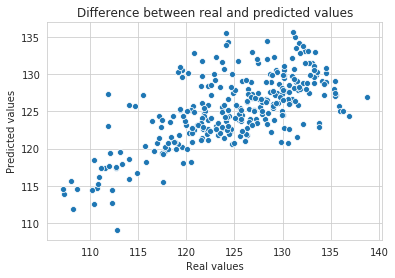
\includegraphics[scale=0.8]{img/output_44_0.png}
\caption{Comparación de los valores reales y los valores predichos.}
\label{fig:comp}
\end{figure}

Como podemos observar, los valores predichos de las etiquetas tienden a
crecer a medida que crecen los valores reales de las etiquetas. Este
crecimiento parece ser lineal, pero al presentar errores en los valores
predichos, no se tiene exactamente un crecimiento lineal perfecto, si no
uno distorsionado. A pesar de esto, los valores predichos no dejan de
estar bastante cerca de los reales.

Como conlusión a este apartado, hemos obtenido un valor de E\(_{test}\)
con el cuál hemos aproximado el valor de E\(_{out}\). Hay que tener en
cuenta que esta es una aproximación, y que el valor de E\(_{out}\) puede
ser incluso muy superior si la muestra que hemos escogido para ajustar
nuestro modelo y la que hemos usado para realizar el test del ajuste no
es representativa de la población (aunque para eso, habría que tener muy
mala suerte). Además, es importante destacar que a medida que se vayan
obteniendo más datos en training, mejor se podrá ajustar el modelo, y
por tanto, el valor de E\(_{out}\) podrá verse reducido aún más (o
incrementado en caso de que nuestro modelo produzca \emph{overfitting}).

    \subsection{Conclusiones finales}\label{conclusiones-finales}

Vamos a cerrar este problema con unas conclusiones finales sobre el
modelo que hemos seleccionado y ajustado posteriormente.

El modelo que hemos seleccionado ha sido el mejor de todos los que hemos
evaluado. Hemos probado con modelos lineales más complejos que
intentaban técnicas más avanzadas como por ejemplo la regularización o
ajustar el mejor hiperplano dentro de un margen. Sin embargo, a pesar de
lo sofisticado de las técnicas, el modelo que ha prevalecido, ante todo
pronóstico, es el más simple, el que no utilizaba ninguna de estas
técnicas. Es posible que, para este problema y para este conjunto de
datos, la regularización no hubiese aportado mucho, ya que no parecía
que hubiese mucha posibilidad de que se produjese \emph{overfitting} al
ajustar una recta (parece que hemos tenido una cantidad de datos
suficiente). Intentar ajustar un hiperplano dentro de un margen es
complicado, ya que hay que considerar bastantes hiperparámetros, como
por ejemplo la anchura del margen o la ponderación que se le asigna al
error de los puntos que caen fuera del margen.

El modelo seleccionado se ha ajustado muy bien a los datos, tanto a la
hora de evaluarlo como en su posterior ajuste con todos los datos de
training. Esto se ha podido observar en el hecho de que el error que de
media se ha obtenido en la evaluación se ha visto reducido
posteriormente en el ajuste con todos los datos. Por tanto, a medida que
proporcionemos más datos a nuestro modelo, más aprenderá y mejor será
capaz de generalizar.

En cuanto a su capacidad de generalizar, tal y como hemos dicho hace un
momento, si seguimos proporcionando datos de entrenamiento al modelo
podemos conseguir que se reduzca más el error fuera de la muestra (hasta
cierto punto, obviamente). Además, tal y como se ve en la figura \ref{fig:comp},
parece que los datos tienen un comportamiento lineal, con lo cuál parece
ser que el ajuste realizado es suficientemente representativo con los
datos de la muestra.

Haber elegido un modelo lineal ha sido una buena idea, ya que con un
número suficiente de datos, podemos obtener un error fuera de la muestra
razonable con una capacidad de generalización buena, aunque podría
quedarse limitado si los datos hubiesen presentado un comportamiento no
lineal.

Es muy posible que al utilizar modelos no lineales nos encontrasemos con
alguno que nos ofreciese unos mejores resultados (un menor error). Sin
embargo, al estar restringidos a modelos lineales, no lo podremos saber
con total seguridad.

Como pequeño resumen, nuestro modelo de Regresión Lineal ha dado muy
buenos resultados en general y es el que mejor desempeño ha tenido de
todos los modelos lineales que hemos probado. Puede ser que haya modelos
no lineales que ofrezcan unos resultados superiores, eso sin dudarlo.
Sin embargo, los resultados obtenidos, a pesar de ser un modelo tan
simple, son muy buenos, y parece que aún queda margen de mejora.

\newpage

\section{\textsc{Problema de Clasificación}}

\subsection{Descripción del problema}\label{descripciuxf3n-del-problema}

    En este problema vamos a trabajar con el conjunto de datos \emph{Optical
Recognition of Handwritten Digits}\cite{digits}. Este conjunto de datos ya ha sido
preprocesado y contiene información sobre distintos dígitos manuscritos.
Cada fila del conjunto de datos contiene 64 valores enteros que se
encuentran en el rango \([0, 16]\) y un valor entero más que se
encuentra en el rango \([0, 9]\), lo cuál se corresponde con el dígito
manuscrito.

El motivo por el que se tienen 64 valores enteros de entrada es que los
datos sin procesar eran \emph{bitmaps} de \(32 \times 32\) bits, en los
que se representaba el dígito manuscrito. Cada bit representaba si se
había escrito en esa posición (valor 1) o no (valor 0). Con el objetivo
de reducir la cantidad de información, el \emph{bitmap} se dividió en
zonas de \(4 \times 4\) bits, y para cada zona, se contaron el número de
bits que tenían valor 1. Al hacer esta división, se obtuvieron 64 zonas
(correspondientes a los 64 valores enteros de entrada), y el número de
bits que podían valer 1 en esa zona iba de 0 a 16.

El conjunto de datos ya viene dividido en un conjunto de training y en
un conjunto de test, con lo cuál no hará falta hacer una división de
éste, cosa que si que pasaba en el anterior problema, donde solo
teníamos un conjunto de datos.

    \subsection{Análisis de los datos}\label{anuxe1lisis-de-los-datos}

    Tal y como hacíamos en el problema anterior, vamos a comenzar con un
análisis de los datos antes de pasar a hablar de qué modelo elegir o qué
clase de funciones utilizar.

Lo primero que tenemos que hacer es cargar los datos, tanto los de
training como los de test. Después de eso obtendremos de forma separada
las características y las etiquetas. Además de eso, para ilustrar mejor
como se representan los datos de entrada, vamos a mostrar los primeros
valores del conjunto de training. Todo esto se puede ver a continuación:

    \begin{Verbatim}[commandchars=\\\{\}]
{\color{incolor}In [{\color{incolor}18}]:} \PY{c+c1}{\PYZsh{} Leer los datos de training y test}
         \PY{n}{train\PYZus{}df} \PY{o}{=} \PY{n}{read\PYZus{}data\PYZus{}values}\PY{p}{(}\PY{l+s+s1}{\PYZsq{}}\PY{l+s+s1}{datos/optdigits.tra}\PY{l+s+s1}{\PYZsq{}}\PY{p}{)}
         \PY{n}{test\PYZus{}df} \PY{o}{=} \PY{n}{read\PYZus{}data\PYZus{}values}\PY{p}{(}\PY{l+s+s1}{\PYZsq{}}\PY{l+s+s1}{datos/optdigits.tes}\PY{l+s+s1}{\PYZsq{}}\PY{p}{)}
         
         \PY{c+c1}{\PYZsh{} Separar las caracteristicas y las etiquetas}
         \PY{n}{X\PYZus{}train}\PY{p}{,} \PY{n}{y\PYZus{}train} \PY{o}{=} \PY{n}{divide\PYZus{}data\PYZus{}labels}\PY{p}{(}\PY{n}{train\PYZus{}df}\PY{p}{)}
         \PY{n}{X\PYZus{}test}\PY{p}{,} \PY{n}{y\PYZus{}test} \PY{o}{=} \PY{n}{divide\PYZus{}data\PYZus{}labels}\PY{p}{(}\PY{n}{test\PYZus{}df}\PY{p}{)}
         
         \PY{c+c1}{\PYZsh{} Mostrar primeros valores del conjunto de training}
         \PY{n}{display}\PY{p}{(}\PY{n}{train\PYZus{}df}\PY{o}{.}\PY{n}{head}\PY{p}{(}\PY{p}{)}\PY{p}{)}
\end{Verbatim}

\begin{figure}[H]
\centering
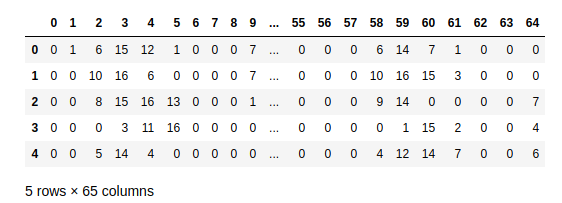
\includegraphics[scale=0.65]{img/train_head_class.png}
\caption{Tabla con las 5 primeras muestras del conjunto de training para el problema de clasificación.}
\end{figure}

Sabiendo esto, a lo mejor nos podría interesar conocer si faltan datos,
los rangos de los valores, etc. Ya sabemos los posibles valores que
puede tomar cada característica y variable de salida, y según el
repositorio no faltan datos, pero nunca está de más comprobar esto
último, así que vamos a hacerlo tanto para el conjunto de training como
para el test. Y ya que estamos, vamos a ver cuántas muestras tenemos en
cada conjunto:

    \begin{Verbatim}[commandchars=\\\{\}]
{\color{incolor}In [{\color{incolor}19}]:} \PY{c+c1}{\PYZsh{} Determinar si faltan valores para los dos conjunts}
         \PY{n+nb}{print}\PY{p}{(}\PY{l+s+s1}{\PYZsq{}}\PY{l+s+s1}{Missing values in train? }\PY{l+s+s1}{\PYZsq{}}\PY{p}{,} \PY{n}{train\PYZus{}df}\PY{o}{.}\PY{n}{isnull}\PY{p}{(}\PY{p}{)}\PY{o}{.}\PY{n}{values}\PY{o}{.}\PY{n}{any}\PY{p}{(}\PY{p}{)}\PY{p}{)}
         \PY{n+nb}{print}\PY{p}{(}\PY{l+s+s1}{\PYZsq{}}\PY{l+s+s1}{Missing values in test? }\PY{l+s+s1}{\PYZsq{}}\PY{p}{,} \PY{n}{test\PYZus{}df}\PY{o}{.}\PY{n}{isnull}\PY{p}{(}\PY{p}{)}\PY{o}{.}\PY{n}{values}\PY{o}{.}\PY{n}{any}\PY{p}{(}\PY{p}{)}\PY{p}{)}
         
         \PY{c+c1}{\PYZsh{} Determinar numero de muestras por conjunto}
         \PY{n+nb}{print}\PY{p}{(}\PY{l+s+s1}{\PYZsq{}}\PY{l+s+s1}{Training sample size: }\PY{l+s+s1}{\PYZsq{}}\PY{p}{,} \PY{n}{train\PYZus{}df}\PY{o}{.}\PY{n}{shape}\PY{p}{[}\PY{l+m+mi}{0}\PY{p}{]}\PY{p}{)}
         \PY{n+nb}{print}\PY{p}{(}\PY{l+s+s1}{\PYZsq{}}\PY{l+s+s1}{Test sample size: }\PY{l+s+s1}{\PYZsq{}}\PY{p}{,} \PY{n}{test\PYZus{}df}\PY{o}{.}\PY{n}{shape}\PY{p}{[}\PY{l+m+mi}{0}\PY{p}{]}\PY{p}{)}
\end{Verbatim}

    \begin{Verbatim}[commandchars=\\\{\}]
Missing values in train?  False
Missing values in test?  False
Training sample size:  3823
Test sample size:  1797

    \end{Verbatim}

    También nos podría interesar saber cómo están distribuidas las clases,
es decir, ver si hay más elementos de una clase que de las otras o si en
cambio están equilibrados. Para visualizarlo, podemos utilizar un
diagrama de barras que nos permita ver cuántos valores de cada clase
hay. Vamos a crear una función que nos permita visualizarlo:

    \begin{Verbatim}[commandchars=\\\{\}]
{\color{incolor}In [{\color{incolor}20}]:} \PY{k}{def} \PY{n+nf}{visualize\PYZus{}distribution}\PY{p}{(}\PY{n}{classes}\PY{p}{,} \PY{n}{values}\PY{p}{,} \PY{n}{columns}\PY{p}{)}\PY{p}{:}
             \PY{l+s+sd}{\PYZdq{}\PYZdq{}\PYZdq{}}
         \PY{l+s+sd}{    Funcion para visualizar en un grafico de barras las}
         \PY{l+s+sd}{    clases con el numero de valores de cada una}
         \PY{l+s+sd}{    }
         \PY{l+s+sd}{    :param classes: Clases que se quieren representar}
         \PY{l+s+sd}{    :param values: Numero de elementos por clase}
         \PY{l+s+sd}{    :param columns: Nombres que dar a las clases y a los}
         \PY{l+s+sd}{                    numeros de elementos al pintar el grafico}
         \PY{l+s+sd}{    \PYZdq{}\PYZdq{}\PYZdq{}}
             
             \PY{c+c1}{\PYZsh{} Crear DataFrame para mostrar el grafico}
             \PY{n}{df\PYZus{}plot} \PY{o}{=} \PY{n}{pd}\PY{o}{.}\PY{n}{DataFrame}\PY{p}{(}\PY{n}{columns}\PY{o}{=}\PY{n}{columns}\PY{p}{,}
                     \PY{n}{data}\PY{o}{=}\PY{p}{[}\PY{p}{[}\PY{n}{v}\PY{p}{,} \PY{n}{l}\PY{p}{]} \PY{k}{for} \PY{n}{v}\PY{p}{,} \PY{n}{l} \PY{o+ow}{in} \PY{n+nb}{zip}\PY{p}{(}\PY{n}{classes}\PY{p}{,} \PY{n}{values}\PY{p}{)}\PY{p}{]}\PY{p}{)}
             
             \PY{c+c1}{\PYZsh{} Crear grafico, poner titulo y mostrar}
             \PY{n}{sns}\PY{o}{.}\PY{n}{barplot}\PY{p}{(}\PY{n}{x}\PY{o}{=}\PY{n}{columns}\PY{p}{[}\PY{l+m+mi}{0}\PY{p}{]}\PY{p}{,} \PY{n}{y}\PY{o}{=}\PY{n}{columns}\PY{p}{[}\PY{l+m+mi}{1}\PY{p}{]}\PY{p}{,} \PY{n}{data}\PY{o}{=}\PY{n}{df\PYZus{}plot}\PY{p}{)}
             \PY{n}{plt}\PY{o}{.}\PY{n}{title}\PY{p}{(}\PY{l+s+s1}{\PYZsq{}}\PY{l+s+s1}{Number of samples per digit class}\PY{l+s+s1}{\PYZsq{}}\PY{p}{)}
             \PY{n}{plt}\PY{o}{.}\PY{n}{show}\PY{p}{(}\PY{p}{)}
\end{Verbatim}

    Y con esto, vamos a visualizar los datos de entrenamiento:

    \begin{Verbatim}[commandchars=\\\{\}]
{\color{incolor}In [{\color{incolor}21}]:} \PY{c+c1}{\PYZsh{} Obtener las clases}
         \PY{n}{classes} \PY{o}{=} \PY{n}{np}\PY{o}{.}\PY{n}{unique}\PY{p}{(}\PY{n}{train\PYZus{}df}\PY{o}{.}\PY{n}{values}\PY{p}{[}\PY{p}{:}\PY{p}{,} \PY{o}{\PYZhy{}}\PY{l+m+mi}{1}\PY{p}{]}\PY{p}{)}
         
         \PY{c+c1}{\PYZsh{} Obtener el numero de muestras por clase}
         \PY{n}{num\PYZus{}elements} \PY{o}{=} \PY{p}{[}\PY{p}{]}
         
         \PY{k}{for} \PY{n}{i} \PY{o+ow}{in} \PY{n}{classes}\PY{p}{:}
             \PY{n}{num\PYZus{}elements}\PY{o}{.}\PY{n}{append}\PY{p}{(}\PY{n}{np}\PY{o}{.}\PY{n}{where}\PY{p}{(}\PY{n}{y\PYZus{}train} \PY{o}{==} \PY{n}{i}\PY{p}{)}\PY{p}{[}\PY{l+m+mi}{0}\PY{p}{]}\PY{o}{.}\PY{n}{shape}\PY{p}{[}\PY{l+m+mi}{0}\PY{p}{]}\PY{p}{)}
         
         \PY{c+c1}{\PYZsh{} Establecer nombres de los ejes [x, y]}
         \PY{n}{axis} \PY{o}{=} \PY{p}{[}\PY{l+s+s1}{\PYZsq{}}\PY{l+s+s1}{digits}\PY{l+s+s1}{\PYZsq{}}\PY{p}{,} \PY{l+s+s1}{\PYZsq{}}\PY{l+s+s1}{num\PYZus{}samples}\PY{l+s+s1}{\PYZsq{}}\PY{p}{]}
         
         \PY{c+c1}{\PYZsh{} Visualizar grafico}
         \PY{n}{visualize\PYZus{}distribution}\PY{p}{(}\PY{n}{classes}\PY{p}{,} \PY{n}{np}\PY{o}{.}\PY{n}{asarray}\PY{p}{(}\PY{n}{num\PYZus{}elements}\PY{p}{)}\PY{p}{,} \PY{n}{axis}\PY{p}{)}
\end{Verbatim}

\begin{figure}[H]
\centering
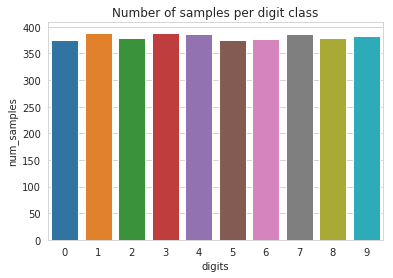
\includegraphics[scale=0.7]{img/output_58_0.png}
\caption{Distribución del número de elementos por clase.}
\end{figure}
    
    Como podemos ver, el número de muestras para cada clase está muy
equilibrado. Hay muy poca variabilidad entre el número de muestras de
cada clase, y por tanto, cada una de ellas está muy bien representada
(no hay una clase que tenga muchísimas más muestras que el resto).

En este problema tenemos demasiadas dimensiones como para poder realizar
un análisis más profundo de los datos. Hacer un análisis de
correlaciones sería un proceso demasiado costoso y engoroso, y por tanto
no será llevado a cabo para este problema. Además, a simple vista, no
parece que exista una auténtica correlación entre ninguna de las
variables de entrada.

Así que, sabiendo que tenemos demasiadas dimensiones en este problema,
la pregunta que nos vamos a hacer es: ¿existe alguna forma de reducir el
número de dimensiones en este problema, sin perder demasiada capacidad
para explicar los datos?

    \subsection{Reducción de
dimensionalidad}\label{reducciuxf3n-de-dimensionalidad}

Para resoponer a la pregunta que nos hemos planteado anteriormente,
vamos a intentar entender mejor lo que queremos conseguir. Nuestro
objetivo es, a partir de los datos que disponemos, encontrar una forma
de \textbf{reducir el número de dimensiones sin perder demasiada
capacidad para explicar la varianza de los datos}. Es decir, queremos
quedarnos con aquellas características que expliquen en mayor medida la
varianza de los datos. Para ello, usaremos una técnica llamada PCA
(Principal Component Analysis) que se basa en la descomposición en SVD.
Con esta técnica transformaremos el espacio en el que estamos trabajando
a uno en el que haya menos dimensiones, conservando un porcentaje alto
de la varianza explicada (en torno a 90-95\%). Cuantas más dimensiones
se reduzcan, menos porcentaje de la varianza podremos explicar, así que
hay que encontrar un equilibrio.

Hemos visto cómo podemos reducir la dimensionalidad. Sin embargo, no
hemos contestado a otra pregunta muy importante: ¿por qué queremos
reducir el número de dimensiones? Aparte de que los tiempos de cómputo
bajarán, hay muchas características que no aportan realmente nada. Por
ejemplo, las zonas del \emph{bitmap} que conforman las esquinas pocas
veces nos vana a dar información de qué dígito es el que se encuentra
representado. También hay otras zonas que no aportan mucha información.
Por tanto, queremos eliminar todas aquellas dimensiones ``inútiles'' que
no sean capaces de ayudarnos a explicar los datos.

Una vez dicho esto, hace falta recalcar unos pequeños detalles. El
primero es que aplicaremos la reducción de dimensionalidad a los datos
de training \textbf{una vez elegido el modelo}, no antes (aplicaremos
eso sí la reducción sobre los datos con los que entrenaremos y
evaluaremos los modelos). El segundo es que PCA es una técnica muy
susceptible a los valores de los datos de entrada. Por tanto, antes de
reducir el número de dimensiones, tendremos que escalar los datos tal y
como se hizo en el problema anterior.

    \subsection{Selección de funciones}\label{selecciuxf3n-de-funciones}

Antes de comentar los modelos que queremos evaluar, vamos a hablar
brevemente de las funciones que utilizaremos.

Tal y como hicimos en el problema anterior, en este caso vamos a
utilizar \textbf{combinaciones lineales} de los datos. No tiene mucho
sentido realizar transformaciones no lineales sobre éstos ya que las
características de los datos de entrada hacen referencia a la cantidad
de valores 1 que hay en una zona del \emph{bitmap}. Por tanto, añadir
por ejemplo los cuadrados de los valores de entrada no parece que nos
vaya a ayudar mucho y tampoco parece tener mucho sentido (¿qué significa
que se eleve al cuadrado el número de bits de una zona?). Otro motivo
muy importante por el que no se aplicarán transformaciones no lineales
es que ya tenemos bastantes dimensiones, con lo cuál añadir más nos
puede llegar a dar problemas (\emph{overfitting}, más tiempo de
entrenamiento, etc.).

\subsection{Selección de métricas}\label{selecciuxf3n-de-muxe9tricas}

El último aspecto que vamos a comentar antes de pasar a hablar de los
modelos que evaluaremos serán las métricas que utilizaremos tanto en el
ajuste de los modelos como en su posterior evaluación.

\subsubsection{Métricas del ajuste}\label{muxe9tricas-del-ajuste}

En el ajuste de los modelos utilizaremos dos métricas:

\begin{itemize}
\item
  \textbf{Cross-Entropy}: utilizaremos esta métrica para el modelo que
  utiliza Regresión Logística Multinomial, ya que es la que normalmente
  se utiliza en los modelos de regresión logística. Como estamos
  trabajando con probabilidades, queremos minimizar el error que se
  comete al intentar predecir que un elemento pertenece a una clase
  determinada, así que esta es la métrica más adecuada en este caso.
\item
  \textbf{Hinge}: utilizaremos esta métrica para el modelo que utiliza
  SVM para clasificación, ya que es la que normalmente se utiliza en
  estos casos, debido a que mide tanto si se predice bien el resultado
  como si se deja margen suficiente.
\end{itemize}

\subsubsection{Métricas de
evaluación}\label{muxe9tricas-de-evaluaciuxf3n}

Para evaluar y comparar los ditintos modelos utilizaremos la precisión
(tasa de aciertos, es decir, la tasa de elementos bien clasificados). El
mejor modelo será el que tenga una precisión mayor que el resto, y
dependiendo de como de alta sea, podremos decir si un modelo es bueno o
malo. Se ha elegido esta métrica debido a que no nos interesa ver el
error que cometemos, si no simplemente si estamos clasificando bien o
no.

Adicionalmente, para el modelo definitivo, se usará también la matriz de
confusión para ver mejor qué clases clasifica mejor que otras, con el
objetivo de simplificar el análisis de los resultados obtenidos.

    \subsection{Selección de modelos}\label{selecciuxf3n-de-modelos}

Pasemos ahora a ver qué modelos vamos a utilizar en este problema. Antes
de comentarlos, hace falta destacar que en este caso no utilizaremos el
\textbf{perceptrón}, debido a que los datos pueden no ser linealmente
separables (no lo sabemos con certeza, pero es probable que así sea) y a
que necesitaríamos una gran cantidad de perceptrones para poder
clasificar bien los datos. Probablemente con un MLP (Multilayer
Perceptron) podríamos obtener unos buenos resultados. Sin embargo,
estamos probando modelos lineales, y entre ellos no se encuentran las
redes neuronales.

Otra cosa que hace falta destacar es que \textbf{todos los modelos
utilizarán regularización}, la cuál será la norma \(\ell 2\). Esto se
debe tanto a que el módulo que estamos utilizando (scikit-learn) no
permite no utilizar regularización como a que en este problema la
regularización puede ofrecer unos mejores resultados, ya que se
intentará restringir el espacio con tal de obtener soluciones de mejor
calidad y evitar el \emph{overfitting}, lo cuál puede darse en este caso
sin que nos demos cuenta con mucha facilidad si por ejemplo las clases
no tienen la misma distribución (no hay un número de elementos similar
en cada clase debido a que casi todos pertenecen a una de ellas, por
ejemplo).

\subsubsection{Regresión Logística
Multinomial}\label{regresiuxf3n-loguxedstica-multinomial}

El primer modelo que evaluaremos será la Regresión Logística
Multinomial, utilizando la función \(softmax\) para obtener las
probabilidades para clasificar. Se ha escogido este modelo porque es la
generalización de la Regresión Logística para más de dos clases, debido
a que solo se entrena un modelo (si usaramos Regresión Logística con
criterio \emph{One vs Rest} estaríamos entrenando múltiples modelos para
ver cuál es el que da una mayor probabilidad de que pertenezca a esa
clase) y debido a que la salida es mucho más interpretable, ya que se
escoge la clases con mayor probabilidad, en vez de que cada modelo diga
cuál es la probabilidad de pertenecer a una clase y cuál es la
probabilidad de pertenecer a cualquiera de las otras.

\subsubsection{\texorpdfstring{SVM con \emph{kernel}
lineal}{SVM con kernel lineal}}\label{svm-con-kernel-lineal}

El segundo modelo que evaluaremos será el SVM con \emph{kernel} lineal.
Hemos escogido este modelo a que se suele utilizar en problemas de
clasificación debido a que busca encontrar la mejor separación entre las
clases, intentando dejar el mayor margen posible entre las clases que
pretende separar y minimizando la suma de las violaciones del margen
(puntos que están entre el plano y el margen, a diferencia de SVM en
regresión, donde se minimizaba los que caían fuera del margen). Esta
última parte es controlada por un parámetro \(C\) que pondera la suma de
los errores, con lo cuál modificándolo se obtendrán unos u otros
resultados. Este parámetro puede considerarse como la cantidad de
regularización que se aplica al modelo, ya que un valor de \(C\) más
grande hará que se ajuste más a los datos limitando el número de puntos
dentro del margen, pero hará que la amplitud de este sea más pequeña, y
por tanto, generalizará peor; mientras que un valor de \(C\) más pequeño
hará que haya más puntos dentro del margen, pero la amplitu del margen
será mayor, con lo cuál puede generalizar mejor.

    \subsection{Elección del mejor
modelo}\label{elecciuxf3n-del-mejor-modelo}

Para elegir el mejor modelo, vamos a llevar a cabo un proceso casi
idéntico al que hemos realizado anteriormente. Con el objetivo de evitar
repetir información, vamos a describir cuál sería el procedimiento,
destacando qué nuevas cosas tendríamos que hacer. Si aparece algún
procedimiento que ya aparecía en el problema anterior, las
justificaciones del por qué son las mismas. Con esto dicho, vamos a ver
como sería el proceso.

Con el conjunto de entrenamiento, realizaremos un \textbf{10-fold
cross-validation} para cada modelo. La principal diferencia en este
problema es que, al tener que clasificar, nos interesaría que las
particiones que se hagan, aparte de ser disjuntas como lo eran en el
problema anterior, tienen que contener un número de elementos de cada
clase proporcional al que hay en la muestra, ya que nos interesa que
cada clase esté proporcionalmente representada en todas las particiones
dependiendo del número de elementos que tenga.

Para cada uno de los folds habrá que escalar los datos con los que se
vaya entrenar el modelo (con el mismo tipo de escalado que hacíamos
antes), entrenar el modelo, escalar los datos con los que se evaluará y
predecir y medir la precisión. Sin embargo, a diferencia del problema
anterior, después de escalar los datos y antes de entrenar se aplicará
la reducción de dimensionalidad con PCA intentando conservar el 95\% de
la varianza explicada.

Finalmente, se escogerá el mejor modelo y se entrenará con todo el
conjunto de entrenamiento, aplicando las transformaciones necesarias. De
ser necesario ajustar algún hiperparámetro, también se hará en este
proceso.

Para cada modelo, vamos a ir probando un conjunto de hiperparámetros y
vamos a ver qué resultados obtenemos en cada caso. Tanto para Regresión
Logística Multinomial como para SVM vamos a probar en cada uno el
parámetro \(C\) (los dos lo tienen por igual) con los valores \(0.01\),
\(0.1\), \(1\) y \(10\) (esto determinará menos o más regularización).

Tal y como hicimos antes, vamos a crear nuestros \textit{pipelines} para cada uno
de los modelos:

\begin{Verbatim}[commandchars=\\\{\}]
{\color{incolor}In [{\color{incolor}22}]:} \PY{c+c1}{\PYZsh{} Clasificador con SVM}
         \PY{k+kn}{from} \PY{n+nn}{sklearn}\PY{n+nn}{.}\PY{n+nn}{svm} \PY{k}{import} \PY{n}{LinearSVC}
         
         \PY{c+c1}{\PYZsh{} Regresion Logistica Multinomial}
         \PY{k+kn}{from} \PY{n+nn}{sklearn}\PY{n+nn}{.}\PY{n+nn}{linear\PYZus{}model} \PY{k}{import} \PY{n}{LogisticRegression}
         
         \PY{c+c1}{\PYZsh{} Metricas de evaluacion}
         \PY{k+kn}{from} \PY{n+nn}{sklearn}\PY{n+nn}{.}\PY{n+nn}{metrics} \PY{k}{import} \PY{n}{accuracy\PYZus{}score}
         \PY{k+kn}{from} \PY{n+nn}{sklearn}\PY{n+nn}{.}\PY{n+nn}{metrics} \PY{k}{import} \PY{n}{confusion\PYZus{}matrix}
         
         \PY{c+c1}{\PYZsh{} k\PYZhy{}fold con proporcion de clases}
         \PY{k+kn}{from} \PY{n+nn}{sklearn}\PY{n+nn}{.}\PY{n+nn}{model\PYZus{}selection} \PY{k}{import} \PY{n}{StratifiedKFold}
         
         \PY{c+c1}{\PYZsh{} Reduccion PCA}
         \PY{k+kn}{from} \PY{n+nn}{sklearn}\PY{n+nn}{.}\PY{n+nn}{decomposition} \PY{k}{import} \PY{n}{PCA}
         
         \PY{k}{def} \PY{n+nf}{create\PYZus{}mlr\PYZus{}pipeline}\PY{p}{(}\PY{n}{c\PYZus{}list}\PY{p}{)}\PY{p}{:}
             \PY{l+s+sd}{\PYZdq{}\PYZdq{}\PYZdq{}}
         \PY{l+s+sd}{    Funcion para crear una lista de pipelines con el}
         \PY{l+s+sd}{    modelo de Regresion Logistica Multinomial dados}
         \PY{l+s+sd}{    unos valores de C, aplicando antes un escalado}
         \PY{l+s+sd}{    y PCA con 95\PYZpc{} de varianza explicada}
         \PY{l+s+sd}{    }
         \PY{l+s+sd}{    :param c\PYZus{}list: Lista de valores C. Un valor por}
         \PY{l+s+sd}{                   cada RLM del pipeline}
         \PY{l+s+sd}{    }
         \PY{l+s+sd}{    :return Devuelve una lista con los pipelines}
         \PY{l+s+sd}{    \PYZdq{}\PYZdq{}\PYZdq{}}
             
             \PY{c+c1}{\PYZsh{} Crear lista de pipelines}
             \PY{n}{pipelines} \PY{o}{=} \PY{p}{[}\PY{p}{]}
             
             \PY{c+c1}{\PYZsh{} Insertar nuevo pipeline}
             \PY{k}{for} \PY{n}{c} \PY{o+ow}{in} \PY{n}{c\PYZus{}list}\PY{p}{:}
                 \PY{n}{pipelines}\PY{o}{.}\PY{n}{append}\PY{p}{(}
                     \PY{n}{make\PYZus{}pipeline}\PY{p}{(}\PY{n}{StandardScaler}\PY{p}{(}\PY{p}{)}\PY{p}{,}
                 	\PY{n}{PCA}\PY{p}{(}\PY{n}{n\PYZus{}components}\PY{o}{=}\PY{l+m+mf}{0.95}\PY{p}{)}\PY{p}{,}
                   \PY{n}{LogisticRegression}\PY{p}{(}\PY{n}{multi\PYZus{}class}\PY{o}{=}\PY{l+s+s1}{\PYZsq{}}\PY{l+s+s1}{multinomial}\PY{l+s+s1}{\PYZsq{}}\PY{p}{,}
                                      \PY{n}{solver}\PY{o}{=}\PY{l+s+s1}{\PYZsq{}}\PY{l+s+s1}{newton\PYZhy{}cg}\PY{l+s+s1}{\PYZsq{}}\PY{p}{,}
                                      \PY{n}{C}\PY{o}{=}\PY{n}{c}\PY{p}{,} \PY{n}{random\PYZus{}state}\PY{o}{=}\PY{l+m+mi}{1}\PY{p}{)}\PY{p}{)}\PY{p}{)}
             
             \PY{k}{return} \PY{n}{pipelines}
         
         \PY{k}{def} \PY{n+nf}{create\PYZus{}svmc\PYZus{}pipeline}\PY{p}{(}\PY{n}{c\PYZus{}list}\PY{p}{)}\PY{p}{:}
             \PY{l+s+sd}{\PYZdq{}\PYZdq{}\PYZdq{}}
         \PY{l+s+sd}{    Funcion para crear una lista de pipelines con el}
         \PY{l+s+sd}{    modelo de SVM dados unos valores de C, aplicando }
         \PY{l+s+sd}{    antes un escalado y PCA con 95\PYZpc{} de varianza explicada}
         \PY{l+s+sd}{    }
         \PY{l+s+sd}{    :param c\PYZus{}list: Lista de valores C. Un valor por}
         \PY{l+s+sd}{                   cada SVM del pipeline}
         \PY{l+s+sd}{    }
         \PY{l+s+sd}{    :return Devuelve una lista con los pipelines}
         \PY{l+s+sd}{    \PYZdq{}\PYZdq{}\PYZdq{}}
             
             \PY{c+c1}{\PYZsh{} Crear lista de pipelines}
             \PY{n}{pipelines} \PY{o}{=} \PY{p}{[}\PY{p}{]}
             
             \PY{c+c1}{\PYZsh{} Insertar nuevo pipeline}
             \PY{k}{for} \PY{n}{c} \PY{o+ow}{in} \PY{n}{c\PYZus{}list}\PY{p}{:}
                 \PY{n}{pipelines}\PY{o}{.}\PY{n}{append}\PY{p}{(}
                     \PY{n}{make\PYZus{}pipeline}\PY{p}{(}\PY{n}{StandardScaler}\PY{p}{(}\PY{p}{)}\PY{p}{,}
                     	      \PY{n}{PCA}\PY{p}{(}\PY{n}{n\PYZus{}components}\PY{o}{=}\PY{l+m+mf}{0.95}\PY{p}{)}\PY{p}{,}
                                   \PY{n}{LinearSVC}\PY{p}{(}\PY{n}{C}\PY{o}{=}\PY{n}{c}\PY{p}{,} \PY{n}{random\PYZus{}state}\PY{o}{=}\PY{l+m+mi}{1}\PY{p}{,}
                                   \PY{n}{loss}\PY{o}{=}\PY{l+s+s1}{\PYZsq{}}\PY{l+s+s1}{hinge}\PY{l+s+s1}{\PYZsq{}}\PY{p}{)}\PY{p}{)}\PY{p}{)}
             
             \PY{k}{return} \PY{n}{pipelines}
\end{Verbatim}

    Vamos a preparar ahora los modelos para poder evaluarlos:
    
\begin{Verbatim}[commandchars=\\\{\}]
{\color{incolor}In [{\color{incolor}23}]:} \PY{c+c1}{\PYZsh{} Crear lista de valores de C para los dos modelos}
         \PY{n}{c\PYZus{}list} \PY{o}{=} \PY{p}{[}\PY{l+m+mf}{0.01}\PY{p}{,} \PY{l+m+mf}{0.1}\PY{p}{,} \PY{l+m+mf}{1.0}\PY{p}{,} \PY{l+m+mf}{10.0}\PY{p}{]}
         
         \PY{c+c1}{\PYZsh{} Crear los nombres de los modelos}
         \PY{n}{model\PYZus{}names} \PY{o}{=} \PY{p}{[}\PY{l+s+s1}{\PYZsq{}}\PY{l+s+s1}{MLR c=0.01}\PY{l+s+s1}{\PYZsq{}}\PY{p}{,} \PY{l+s+s1}{\PYZsq{}}\PY{l+s+s1}{MLR c=0.1}\PY{l+s+s1}{\PYZsq{}}\PY{p}{,}
                        \PY{l+s+s1}{\PYZsq{}}\PY{l+s+s1}{MLR c=1.0}\PY{l+s+s1}{\PYZsq{}}\PY{p}{,} \PY{l+s+s1}{\PYZsq{}}\PY{l+s+s1}{MLR c=10.0}\PY{l+s+s1}{\PYZsq{}}\PY{p}{,}
                        \PY{l+s+s1}{\PYZsq{}}\PY{l+s+s1}{SVMC c=0.01}\PY{l+s+s1}{\PYZsq{}}\PY{p}{,} \PY{l+s+s1}{\PYZsq{}}\PY{l+s+s1}{SVMC c=0.1}\PY{l+s+s1}{\PYZsq{}}\PY{p}{,}
                        \PY{l+s+s1}{\PYZsq{}}\PY{l+s+s1}{SVMC c=1.0}\PY{l+s+s1}{\PYZsq{}}\PY{p}{,} \PY{l+s+s1}{\PYZsq{}}\PY{l+s+s1}{SVMC c=10.0}\PY{l+s+s1}{\PYZsq{}}\PY{p}{]}
         
         \PY{c+c1}{\PYZsh{} Crear 10\PYZhy{}fold que conserva la proporcion}
         \PY{n}{cv} \PY{o}{=} \PY{n}{StratifiedKFold}\PY{p}{(}\PY{n}{n\PYZus{}splits}\PY{o}{=}\PY{l+m+mi}{10}\PY{p}{,} \PY{n}{shuffle}\PY{o}{=}\PY{k+kc}{True}\PY{p}{,} \PY{n}{random\PYZus{}state}\PY{o}{=}\PY{l+m+mi}{1}\PY{p}{)}
         
         \PY{c+c1}{\PYZsh{} Crear pipelines para cada modelo}
         \PY{n}{mlr\PYZus{}pipe} \PY{o}{=} \PY{n}{create\PYZus{}mlr\PYZus{}pipeline}\PY{p}{(}\PY{n}{c\PYZus{}list}\PY{p}{)}
         \PY{n}{svmc\PYZus{}pipe} \PY{o}{=} \PY{n}{create\PYZus{}svmc\PYZus{}pipeline}\PY{p}{(}\PY{n}{c\PYZus{}list}\PY{p}{)}
         
         \PY{c+c1}{\PYZsh{} Juntar todos los pipelines en una lista con los modelos}
         \PY{n}{models} \PY{o}{=} \PY{n}{mlr\PYZus{}pipe} \PY{o}{+} \PY{n}{svmc\PYZus{}pipe}
\end{Verbatim}

    Y con todo listo, vamos a observar los resultados que nos ofrece cada
uno de los modelos que estamos evaluando:

\begin{Verbatim}[commandchars=\\\{\}]
{\color{incolor}In [{\color{incolor}24}]:} \PY{k+kn}{import} \PY{n+nn}{warnings}
         \PY{n}{warnings}\PY{o}{.}\PY{n}{filterwarnings}\PY{p}{(}\PY{l+s+s1}{\PYZsq{}}\PY{l+s+s1}{ignore}\PY{l+s+s1}{\PYZsq{}}\PY{p}{)}
         
         \PY{c+c1}{\PYZsh{} Obtener valores medios y desviaciones de las evaluaciones}
         \PY{n}{means}\PY{p}{,} \PY{n}{deviations} \PY{o}{=} \PY{n}{evaluate\PYZus{}models}\PY{p}{(}\PY{n}{models}\PY{p}{,} \PY{n}{X\PYZus{}train}\PY{p}{,} \PY{n}{y\PYZus{}train}\PY{p}{,}
                                             \PY{n}{cv}\PY{o}{=}\PY{n}{cv}\PY{p}{,} \PY{n}{metric}\PY{o}{=}\PY{l+s+s1}{\PYZsq{}}\PY{l+s+s1}{accuracy}\PY{l+s+s1}{\PYZsq{}}\PY{p}{)}
         
         \PY{c+c1}{\PYZsh{} Mostrar valores por pantalla}
         \PY{n}{print\PYZus{}evaluation\PYZus{}results}\PY{p}{(}\PY{n}{model\PYZus{}names}\PY{p}{,} \PY{n}{means}\PY{p}{,} \PY{n}{deviations}\PY{p}{,}
         			 \PY{l+s+s1}{\PYZsq{}}\PY{l+s+s1}{Mean Accuracy}\PY{l+s+s1}{\PYZsq{}}\PY{p}{)}
\end{Verbatim}

    \begin{Verbatim}[commandchars=\\\{\}]
Evaluation results for each model

    \end{Verbatim}

\begin{figure}[H]
\centering
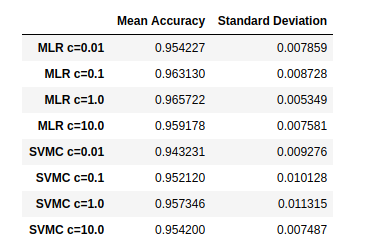
\includegraphics[scale=0.7]{img/evaluations_class.png}
\end{figure}

Observando los resultados, podemos ver que la Regresión Logística
Multinomial que utiliza \(C = 1\) es la que ofrece una mejor precisión
media junto con una menor desviación típica en los resultados. Esto se
debe a que cuanto más pequeño sea el valor de \(C\), mayor será la
regularización que se aplique. Al tener que \(C = 1\) se pondera el
error de manera neutra, sin darle más o menos importancia a éste. A
medida que va aumentando el valor de \(C\), los resultados que se
obtienen parecen empeorar ya que se aplica menos regularización. Por
tanto, parece ser que o bien se aplica una regularización con un valor
neutro, o bien con un valor de \(C\) pequeño que se encuentre en el
rango \([0.1, 1]\), ya que parece que alrededor de estos valores se
obtienen buenos resultados.

Si miramos al SVM vemos que obtiene unos resultados que de media son
peores que cualquiera de los obtenidos por Regresión Logística
Multinomial, lo cuál no quiere decir que los resultados sean malos, si
no todo lo contrario, son muy buenos, pero la Regresión Logística
Multinomial le gana en una pequeña proporción en cada caso. Esto puede
deberse a que en este problema los datos no sean completamente
linealmente separables o que los vectores soporte de cada clase estén
muy juntos unos de otros, con lo cuál intentar encontrar el mejor
hiperplano que separa una clase del resto parece ser un trabajo difícil,
ya que siempre habrán datos que caigan dentro del margen y harán que el
separador no esté a una buena distancia entre las dos clases.

Por tanto, a la vista de los resultados que hemos obtenido, vamos elegir
como modelo la Regresión Logística Multinomial con \(C = 1\). Se podrían
mejorar los resultados intentando ajustar mejor el valor de \(C\). Sin
embargo, consideramos que no es necesario hacerlo, ya que los resultados
que tenemos son lo suficientemente buenos.

    \subsection{Ajuste del modelo
seleccionado}\label{ajuste-del-modelo-seleccionado}

Una vez elegido nuestro modelo (Regresión Logística Multinomial), vamos
a ajustar el modelo con todos los datos de training.

Para comenzar el proceso, necesitamos primero escalar los datos
utilizando por ejemplo un \emph{StandardScaler}, tal y como hemos hecho
en el problema anterior y cuyo funcionamiento ya se supone conocido. Por
tanto, vamos a hacerlo con el siguiente código:

    \begin{Verbatim}[commandchars=\\\{\}]
{\color{incolor}In [{\color{incolor}25}]:} \PY{c+c1}{\PYZsh{} Creamos un nuevo scaler}
         \PY{n}{scaler} \PY{o}{=} \PY{n}{StandardScaler}\PY{p}{(}\PY{p}{)}
         
         \PY{c+c1}{\PYZsh{} Entrenamos el scaler y transformamos los datos}
         \PY{n}{scaler}\PY{o}{.}\PY{n}{fit}\PY{p}{(}\PY{n}{X\PYZus{}train}\PY{p}{)}
         \PY{n}{X\PYZus{}train} \PY{o}{=} \PY{n}{scaler}\PY{o}{.}\PY{n}{transform}\PY{p}{(}\PY{n}{X\PYZus{}train}\PY{p}{)}
\end{Verbatim}

    Lo que vamos a hacer a continuación es aplicar PCA sobre los datos
transformados y ver cuántas dimensiones se reducen conservando el 95\%
de la varianza explicada:

    \begin{Verbatim}[commandchars=\\\{\}]
{\color{incolor}In [{\color{incolor}26}]:} \PY{c+c1}{\PYZsh{} Creamos un nuevo objeto de PCA}
         \PY{n}{pca} \PY{o}{=} \PY{n}{PCA}\PY{p}{(}\PY{n}{n\PYZus{}components}\PY{o}{=}\PY{l+m+mf}{0.95}\PY{p}{)}
         
         \PY{n+nb}{print}\PY{p}{(}\PY{l+s+s1}{\PYZsq{}}\PY{l+s+s1}{Dimensions before PCA: }\PY{l+s+s1}{\PYZsq{}}\PY{p}{,} \PY{n}{X\PYZus{}train}\PY{o}{.}\PY{n}{shape}\PY{p}{[}\PY{l+m+mi}{1}\PY{p}{]}\PY{p}{)}
         
         \PY{c+c1}{\PYZsh{} Ajustamos PCA y transformamos}
         \PY{n}{pca}\PY{o}{.}\PY{n}{fit}\PY{p}{(}\PY{n}{X\PYZus{}train}\PY{p}{)}
         \PY{n}{X\PYZus{}train} \PY{o}{=} \PY{n}{pca}\PY{o}{.}\PY{n}{transform}\PY{p}{(}\PY{n}{X\PYZus{}train}\PY{p}{)}
         
         \PY{n+nb}{print}\PY{p}{(}\PY{l+s+s1}{\PYZsq{}}\PY{l+s+s1}{Dimensions after PCA: }\PY{l+s+s1}{\PYZsq{}}\PY{p}{,} \PY{n}{X\PYZus{}train}\PY{o}{.}\PY{n}{shape}\PY{p}{[}\PY{l+m+mi}{1}\PY{p}{]}\PY{p}{)}
\end{Verbatim}

    \begin{Verbatim}[commandchars=\\\{\}]
Dimensions before PCA:  64
Dimensions after PCA:  41

    \end{Verbatim}

    Como podemos ver, el número de dimensiones se ha visto reducido en
aproximadamente un 35\% conservando un 95\% de la varianza explicada, lo
cuál es una muy buena reducción sin perder mucha capacidad de explicar
los datos.

Ahora, vamos a ajustar nuestro modelo, recordando que el \(C\) que
utilizamos es \(1\), ya que es el que mejores resultados ha ofrecido a la hora de evaluar. Por defecto, scikit-learn utiliza \(C = 1.0\), así
que no vamos a especificarlo. También es necesario destacar que, por
defecto, el método de resolución que utiliza \emph{LogisticRegression}
no vale para el problema multinomial, con lo cuál tenemos que
especificar otro, aunque eso ya son detalles de implementación. Sin más
dilación, vamos a ajustar nuestro modelo:

    \begin{Verbatim}[commandchars=\\\{\}]
{\color{incolor}In [{\color{incolor}27}]:} \PY{c+c1}{\PYZsh{} Crear modelo}
         \PY{n}{mlr} \PY{o}{=} \PY{n}{LogisticRegression}\PY{p}{(}\PY{n}{multi\PYZus{}class}\PY{o}{=}\PY{l+s+s1}{\PYZsq{}}\PY{l+s+s1}{multinomial}\PY{l+s+s1}{\PYZsq{}}\PY{p}{,}
                                  \PY{n}{solver}\PY{o}{=}\PY{l+s+s1}{\PYZsq{}}\PY{l+s+s1}{newton\PYZhy{}cg}\PY{l+s+s1}{\PYZsq{}}\PY{p}{,} \PY{n}{random\PYZus{}state}\PY{o}{=}\PY{l+m+mi}{1}\PY{p}{)}
         
         \PY{c+c1}{\PYZsh{} Ajustar el modelo}
         \PY{n}{mlr}\PY{o}{.}\PY{n}{fit}\PY{p}{(}\PY{n}{X\PYZus{}train}\PY{p}{,} \PY{n}{y\PYZus{}train}\PY{p}{)}
\end{Verbatim}

            
    Y con esto, ya tenemos nuestro modelo ajustado. Ahora solo nos queda
estimar el error fuera de la muestra.

\subsection{\texorpdfstring{Estimación de
E\(_{out}\)}{Estimación de E\_\{out\}}}\label{estimaciuxf3n-de-e_out}

Vamos a estimar E\(_{out}\) tal y como hicimos en el problema anterior,
mediante E\(_{test}\). En este caso, los errores no son tanto de ver
cómo nos alejamos del valor real, ya que estamos en un problema de
clasificación. Lo que nos interesa es ver qué proporción de los datos
clasificamos correctamente, y aquellos que no clasifiquemos bien serán
los que contribuyan al error. Además, sabiendo que E\(_{test}\) es una
buena cota para E\(_{out}\), podremos decir con bastante certeza que, de
llegar nuevos datos, cometeríamos un error parecido al que hemos
cometido con los datos de test.

Sin demorarnos mucho más, vamos predecir las clases y a obtener el valor
de precisión. Es importante recalcar que, tal y como hicimos en el caso
anterior, tenemos que normalizar y reducir los datos de test.

    \begin{Verbatim}[commandchars=\\\{\}]
{\color{incolor}In [{\color{incolor}28}]:} \PY{c+c1}{\PYZsh{} Escalar y reducir dimensiones en test}
         \PY{n}{X\PYZus{}test\PYZus{}scal} \PY{o}{=} \PY{n}{scaler}\PY{o}{.}\PY{n}{transform}\PY{p}{(}\PY{n}{X\PYZus{}test}\PY{p}{)}
         \PY{n}{X\PYZus{}test\PYZus{}red} \PY{o}{=} \PY{n}{pca}\PY{o}{.}\PY{n}{transform}\PY{p}{(}\PY{n}{X\PYZus{}test\PYZus{}scal}\PY{p}{)}
         
         \PY{c+c1}{\PYZsh{} Predecir las etiquetas}
         \PY{n}{y\PYZus{}pred} \PY{o}{=} \PY{n}{mlr}\PY{o}{.}\PY{n}{predict}\PY{p}{(}\PY{n}{X\PYZus{}test\PYZus{}red}\PY{p}{)}
         
         \PY{c+c1}{\PYZsh{} Obtener la precision}
         \PY{n}{accuracy} \PY{o}{=} \PY{n}{accuracy\PYZus{}score}\PY{p}{(}\PY{n}{y\PYZus{}test}\PY{p}{,} \PY{n}{y\PYZus{}pred}\PY{p}{)}
         
         \PY{c+c1}{\PYZsh{} Mostrar valor de la precision}
         \PY{n+nb}{print}\PY{p}{(}\PY{l+s+s1}{\PYZsq{}}\PY{l+s+s1}{Accuracy score: }\PY{l+s+s1}{\PYZsq{}}\PY{p}{,} \PY{n}{accuracy}\PY{p}{)}
\end{Verbatim}

    \begin{Verbatim}[commandchars=\\\{\}]
Accuracy score:  0.9421257651641625

    \end{Verbatim}

    Como podemos comprobar, el valor de precisión que hemos obtenido es de
\(0.94\). Esto significa que nuestro modelo ha acertado al predecir el
94\% de las etiquetas, y que por tanto, ha cometido un \textbf{6\% de
error} al predecir algunas de ellas. Este resultado es un poco peor que
el que obtuvimos al evaluar el modelo, ya que la cantidad de etiquetas
que intentabamos predecir a la hora de evaluar era una décima parte de
la muestra de entrenamiento para cada fold, mientras que aquí tenemos
muchas más. Con lo cuál, al tener aquí más etiquetas que predecir, es
normal que el error se vea incrementado un poco. Sin embargo, que el
error se haya visto incrementado no significa que nuestro modelo sea
malo a la hora de predecir, si no todo lo contrario. Tener más de un
90\% de precisión en un problema de clasificación con 10 clases y más de
40 dimensiones efectivas es una gran hazaña.

Para intentar ver un poco mejor donde se han producido los errores,
vamos a ver la matriz de confusión:

    \begin{Verbatim}[commandchars=\\\{\}]
{\color{incolor}In [{\color{incolor}29}]:} \PY{c+c1}{\PYZsh{} Mostar matriz de confusion}
         \PY{n+nb}{print}\PY{p}{(}\PY{l+s+s1}{\PYZsq{}}\PY{l+s+s1}{Confusion matrix}\PY{l+s+s1}{\PYZsq{}}\PY{p}{)}
         \PY{n+nb}{print}\PY{p}{(}\PY{n}{confusion\PYZus{}matrix}\PY{p}{(}\PY{n}{y\PYZus{}test}\PY{p}{,} \PY{n}{y\PYZus{}pred}\PY{p}{)}\PY{p}{)}
\end{Verbatim}

    \begin{Verbatim}[commandchars=\\\{\}]
Confusion matrix
[[174   0   0   0   0   4   0   0   0   0]
 [  0 173   0   0   0   0   3   0   2   4]
 [  0   5 168   2   0   0   2   0   0   0]
 [  1   0   5 170   0   2   0   0   3   2]
 [  0   2   0   0 174   0   0   1   3   1]
 [  0   0   0   0   0 180   0   0   0   2]
 [  0   0   0   0   3   0 177   0   1   0]
 [  0   0   0   0   2   7   0 160   1   9]
 [  0  11   0   1   0   2   0   0 153   7]
 [  0   1   0   1   5   3   0   0   6 164]]

    \end{Verbatim}

    Para entender la matriz de confusión, tenemos que saber lo que
representa cada eje. El eje horizontal representa los valores que el
modelo ha predicho, mientras que el eje vertical se corresponde con los
valores reales de las etiquetas. Los dos ejes están ordenados, por tanto
no habrá problema en leer los resultados.

Mediante la matriz de confusión podemos ver que tal y como habíamos
dicho hace un momento, nuestro modelo comete errores, ya que no hemos
obtenido una matriz diagonal (de ser así, tendría una precisión del
100\%). Vemos que por ejemplo nuestro modelo comete bastantes errores al
intentar predecir el 8, ya que, a pesar de haber acertado 153 casos, ha
fallado en 11 al considerarlo como un 1. Esto puede extrañar un poco, ya
que los valores 1 y 8 no son muy parecidos, pero probablemente lo que
haya sucedido es que, al aplicar la reducción de dimensionalidad, se
haya eliminado alguna característica que permitía distinguir mejor entre
estas dos clases. Para el resto de clases reales también se cometen
errores al predecir las etiquetas. Las clases donde más número de
errores se han cometido son las clases del 7, el 8 y el 9, con 19, 21 y
16 errores respectivamente. Donde menos, en las clases del 0, 5 y 6, con
4, 2 y 4 errores respectivamente. Todo esto, como hemos comentado hace
un momento, puede deberse a que PCA haya eliminado alguna característica
que permita distinguir algunas clases ya que a lo mejor esa zona tenía
unos valores que de media se acercaban a 0, por ejemplo. Además, esto es
un indicador de que hay que tener cuidado al reducir el número de
dimensiones, ya que se pueden perder características que en un principio
parecían no explicar mucha varianza pero que finalmente sí que fuesen
vitales para permitir distinguir entre algunas clases. Por tanto, de
aquí podemos extraer que PCA es una buena técnica para reducir el número
de dimensiones, pero hay que hacerlo con cuidado para evitar que se
cometan demasiados errores.

    \subsection{Conclusiones finales}\label{conclusiones-finales}

Para conlcuir este proceso de análisis, elección y ajuste de modelo y estimación
del error fuera de la muestra, vamos a sacar unas pequeñas conclusiones sobre nuestro
modelo.

Hemos comparado la Regresión Logística Multinomial con un SVM con
\emph{kernel} lineal utilizando un modelo de evaluación basado en
\textbf{10-fold cross-validation} y hemos obtenido que la regresión
logística ofrecía unos mejores resultados al tener una mayor precisión
media.

Hemos ajustado nuestro modelo después de haber escalado los datos y
aplicarles una reducción de PCA conservando el 95\% de la varianza
explicada, y hemos obtenido una precisión de \(0.94\), valor que está
muy bien teniendo en cuenta que esta vez intentabamos predecir muchas
más etiquetas que durante la evaluación.

Nuestro modelo, a pesar de haber cometido algunos errores a la hora de
predecir las etiquetas de test, ha demostrado que es robusto y que es
capaz de generalizar muy bien, ya que, con los datos con los que que ha
sido ajustado ha sido capaz de predecir correctamente la clase del 94\%
de las 1797 muestras de test.

Por tanto, la Regresión Logística Multinomial ha sido un muy buen modelo
que nos ha permitido obtener muy buenos resultados. Otros modelos que no
son lineales, como por ejemplo el KNN, han conseguido, según los datos
extraídos del reopositorio, una precisión mayor que la que ha obtenido
nuestro modelo. Sin embargo, al ser modelos no lineales, no se han
tenido en cuenta. Y además, para ser un modelo lineal, la Regresión
Logística Multinomial se ha mostrado capaz de hacerle frente a modelos
que en un principio parecen ser más potentes como es el caso del KNN.
Con lo cuál, el modelo que hemos escogido ha sido, de entre los que se
han probado, el más adecuado al problema.

\newpage

\begin{thebibliography}{22}

\bibitem{airfoil}
UCI. \textit{Airfoil Self-Noise Data Set}
\\\url{https://archive.ics.uci.edu/ml/datasets/airfoil+self-noise#}

\bibitem{digits}
UCI. \textit{Optical Recognition of Handwritten Digits Data Set}
\\\url{https://archive.ics.uci.edu/ml/datasets/optical+recognition+of+handwritten+digits}

\bibitem{pca}
Scikit-Learn. \textit{PCA}
\\\url{https://scikit-learn.org/stable/modules/generated/sklearn.decomposition.PCA.html}

\bibitem{scaler}
Scikit-Learn. \textit{StandardScaler}
\\\url{https://scikit-learn.org/stable/modules/generated/sklearn.preprocessing.StandardScaler.html}

\bibitem{pearson}
Wikipedia. \textit{Coeficiente de correlación de Pearson}
\\\url{https://en.wikipedia.org/wiki/Pearson_correlation_coefficient}

\bibitem{linear-models}
Scikit-Learn. \textit{1.1. Generalized Linear Models}
\\\url{https://scikit-learn.org/stable/modules/linear_model.html}

\bibitem{linear-regression}
Scikit-Learn. \textit{LinearRegression}
\\\url{https://scikit-learn.org/stable/modules/generated/sklearn.linear_model.LinearRegression.html#sklearn.linear_model.LinearRegression}

\bibitem{ridge}
Scikit-Learn. \textit{Ridge}
\\\url{https://scikit-learn.org/stable/modules/generated/sklearn.linear_model.Ridge.html#sklearn.linear_model.Ridge}

\bibitem{linear-svr}
Scikit-Learn. \textit{LinearSVR}
\\\url{https://scikit-learn.org/stable/modules/generated/sklearn.svm.LinearSVR.html#sklearn.svm.LinearSVR}

\bibitem{pipeline}
Scikit-Learn. \textit{Pipeline}
\\\url{https://scikit-learn.org/stable/modules/generated/sklearn.pipeline.Pipeline.html}

\bibitem{make-pipeline}
Scikit-Learn. \textit{make\_pipeline}
\\\url{https://scikit-learn.org/stable/modules/generated/sklearn.pipeline.make_pipeline.html}

\bibitem{model-evaluation}
Scikit-Learn. \textit{3.3. Model evaluation: quantifying the quality of predictions}
\\\url{https://scikit-learn.org/stable/modules/model_evaluation.html}

\bibitem{svm}
Scikit-Learn. \textit{1.4. Support Vector Machines}
\\\url{https://scikit-learn.org/stable/modules/svm.html}

\bibitem{regularization}
Anuja Nagpal. \textit{L1 and L2 Regularization Methods}
\\\url{https://towardsdatascience.com/l1-and-l2-regularization-methods-ce25e7fc831c}

\bibitem{logistic-regression}
Scikit-Learn. \textit{LogisticRegression}
\\\url{https://scikit-learn.org/stable/modules/generated/sklearn.linear_model.LogisticRegression.html}

\bibitem{svc}
Scikit-Learn. \textit{LinearSVC}
\\\url{https://scikit-learn.org/stable/modules/generated/sklearn.svm.LinearSVC.html#sklearn.svm.LinearSVC}

\bibitem{scaling}
Scikit-Learn. \textit{Importance of Feature Scaling}
\\\url{https://scikit-learn.org/stable/auto_examples/preprocessing/plot_scaling_importance.html}

\bibitem{accuracy}
Scikit-Learn. \textit{accuracy\_score}
\\\url{https://scikit-learn.org/stable/modules/generated/sklearn.metrics.accuracy_score.html}

\bibitem{mae}
Scikit-Learn. \textit{mean\_absolute\_error}
\\\url{https://scikit-learn.org/stable/modules/generated/sklearn.metrics.mean_absolute_error.html}

\bibitem{confusion-sci}
Scikit-Learn. \textit{confusion\_matrix}
\\\url{https://scikit-learn.org/stable/modules/generated/sklearn.metrics.confusion_matrix.html}

\bibitem{confusion}
Wikipedia. \textit{Confusion matrix}
\\\url{https://en.wikipedia.org/wiki/Confusion_matrix}

\end{thebibliography}

\end{document}

